\documentclass[12pt,]{article}
\usepackage{lmodern}
\let\savedparagraph\paragraph % Save pandoc's definition of paragraph 
\let\paragraph\oldparagraph % Give the old definition that titlesec likes

\let\savedsubparagraph\subparagraph % Same thing for subparagraph 
\let\subparagraph\oldsubparagraph 

% load titlesec
\usepackage[compact]{titlesec}
\newcommand{\sectionbreak}{\clearpage}

\let\paragraph\savedparagraph % Reset to the correct definition
\let\subparagraph\savedsubparagraph % Reset to the correct definition
\usepackage{amssymb,amsmath}
\usepackage{ifxetex,ifluatex}
\usepackage{fixltx2e} % provides \textsubscript
\ifnum 0\ifxetex 1\fi\ifluatex 1\fi=0 % if pdftex
  \usepackage[T1]{fontenc}
  \usepackage[utf8]{inputenc}
\else % if luatex or xelatex
  \ifxetex
    \usepackage{mathspec}
  \else
    \usepackage{fontspec}
  \fi
  \defaultfontfeatures{Ligatures=TeX,Scale=MatchLowercase}
\fi
% use upquote if available, for straight quotes in verbatim environments
\IfFileExists{upquote.sty}{\usepackage{upquote}}{}
% use microtype if available
\IfFileExists{microtype.sty}{%
\usepackage[]{microtype}
\UseMicrotypeSet[protrusion]{basicmath} % disable protrusion for tt fonts
}{}
\PassOptionsToPackage{hyphens}{url} % url is loaded by hyperref
\usepackage[unicode=true]{hyperref}
\hypersetup{
            pdftitle={Accelerated Sensor Fusion for Drones and a Simulation Framework for Spatial},
            pdfauthor={Ruben Fiszel},
            pdfborder={0 0 0},
            breaklinks=true}
\urlstyle{same}  % don't use monospace font for urls
\usepackage[a4paper]{geometry}
\usepackage{color}
\usepackage{fancyvrb}
\newcommand{\VerbBar}{|}
\newcommand{\VERB}{\Verb[commandchars=\\\{\}]}
\DefineVerbatimEnvironment{Highlighting}{Verbatim}{commandchars=\\\{\}}
% Add ',fontsize=\small' for more characters per line
\usepackage{framed}
\definecolor{shadecolor}{RGB}{248,248,248}
\newenvironment{Shaded}{\begin{snugshade}}{\end{snugshade}}
\newcommand{\KeywordTok}[1]{\textcolor[rgb]{0.13,0.29,0.53}{\textbf{#1}}}
\newcommand{\DataTypeTok}[1]{\textcolor[rgb]{0.13,0.29,0.53}{#1}}
\newcommand{\DecValTok}[1]{\textcolor[rgb]{0.00,0.00,0.81}{#1}}
\newcommand{\BaseNTok}[1]{\textcolor[rgb]{0.00,0.00,0.81}{#1}}
\newcommand{\FloatTok}[1]{\textcolor[rgb]{0.00,0.00,0.81}{#1}}
\newcommand{\ConstantTok}[1]{\textcolor[rgb]{0.00,0.00,0.00}{#1}}
\newcommand{\CharTok}[1]{\textcolor[rgb]{0.31,0.60,0.02}{#1}}
\newcommand{\SpecialCharTok}[1]{\textcolor[rgb]{0.00,0.00,0.00}{#1}}
\newcommand{\StringTok}[1]{\textcolor[rgb]{0.31,0.60,0.02}{#1}}
\newcommand{\VerbatimStringTok}[1]{\textcolor[rgb]{0.31,0.60,0.02}{#1}}
\newcommand{\SpecialStringTok}[1]{\textcolor[rgb]{0.31,0.60,0.02}{#1}}
\newcommand{\ImportTok}[1]{#1}
\newcommand{\CommentTok}[1]{\textcolor[rgb]{0.56,0.35,0.01}{\textit{#1}}}
\newcommand{\DocumentationTok}[1]{\textcolor[rgb]{0.56,0.35,0.01}{\textbf{\textit{#1}}}}
\newcommand{\AnnotationTok}[1]{\textcolor[rgb]{0.56,0.35,0.01}{\textbf{\textit{#1}}}}
\newcommand{\CommentVarTok}[1]{\textcolor[rgb]{0.56,0.35,0.01}{\textbf{\textit{#1}}}}
\newcommand{\OtherTok}[1]{\textcolor[rgb]{0.56,0.35,0.01}{#1}}
\newcommand{\FunctionTok}[1]{\textcolor[rgb]{0.00,0.00,0.00}{#1}}
\newcommand{\VariableTok}[1]{\textcolor[rgb]{0.00,0.00,0.00}{#1}}
\newcommand{\ControlFlowTok}[1]{\textcolor[rgb]{0.13,0.29,0.53}{\textbf{#1}}}
\newcommand{\OperatorTok}[1]{\textcolor[rgb]{0.81,0.36,0.00}{\textbf{#1}}}
\newcommand{\BuiltInTok}[1]{#1}
\newcommand{\ExtensionTok}[1]{#1}
\newcommand{\PreprocessorTok}[1]{\textcolor[rgb]{0.56,0.35,0.01}{\textit{#1}}}
\newcommand{\AttributeTok}[1]{\textcolor[rgb]{0.77,0.63,0.00}{#1}}
\newcommand{\RegionMarkerTok}[1]{#1}
\newcommand{\InformationTok}[1]{\textcolor[rgb]{0.56,0.35,0.01}{\textbf{\textit{#1}}}}
\newcommand{\WarningTok}[1]{\textcolor[rgb]{0.56,0.35,0.01}{\textbf{\textit{#1}}}}
\newcommand{\AlertTok}[1]{\textcolor[rgb]{0.94,0.16,0.16}{#1}}
\newcommand{\ErrorTok}[1]{\textcolor[rgb]{0.64,0.00,0.00}{\textbf{#1}}}
\newcommand{\NormalTok}[1]{#1}
\usepackage{graphicx,grffile}
\makeatletter
\def\maxwidth{\ifdim\Gin@nat@width>\linewidth\linewidth\else\Gin@nat@width\fi}
\def\maxheight{\ifdim\Gin@nat@height>\textheight\textheight\else\Gin@nat@height\fi}
\makeatother
% Scale images if necessary, so that they will not overflow the page
% margins by default, and it is still possible to overwrite the defaults
% using explicit options in \includegraphics[width, height, ...]{}
\setkeys{Gin}{width=\maxwidth,height=\maxheight,keepaspectratio}
\IfFileExists{parskip.sty}{%
\usepackage{parskip}
}{% else
\setlength{\parindent}{0pt}
\setlength{\parskip}{6pt plus 2pt minus 1pt}
}
\setlength{\emergencystretch}{3em}  % prevent overfull lines
\providecommand{\tightlist}{%
  \setlength{\itemsep}{0pt}\setlength{\parskip}{0pt}}
\setcounter{secnumdepth}{5}
% Redefines (sub)paragraphs to behave more like sections
\ifx\paragraph\undefined\else
\let\oldparagraph\paragraph
\renewcommand{\paragraph}[1]{\oldparagraph{#1}\mbox{}}
\fi
\ifx\subparagraph\undefined\else
\let\oldsubparagraph\subparagraph
\renewcommand{\subparagraph}[1]{\oldsubparagraph{#1}\mbox{}}
\fi

% set default figure placement to htbp
\makeatletter
\def\fps@figure{htbp}
\makeatother


\begin{document}

%% Template for the title page of the thesis

\begin{titlepage}
\begin{center}
\Large
\textbf{École Polytechnique Fédérale de Lausanne} \\
\vspace{1cm}
Master Thesis
\vspace{2cm}
\hrule
\vspace{0.1cm}
\hrule
\vspace{1cm}
\Huge
\textbf{Accelerated Sensor Fusion for Drones and a Simulation Framework for
Spatial}
\vspace{1cm}
\hrule
\vspace{0.1cm}
\hrule
\end{center}
\vfill
\noindent \textbf{Author} \hfill \textbf{August 29, 2017} \\
Ruben Fiszel \\
\textit{ruben.fiszel@epfl.ch} \\
\vspace{0.5cm}

\noindent \textbf{Supervisors} \\
Prof. Martin Odersky            \hfill    Prof. Oyekunle A. Olukotun \\
LAMP | EPFL                     \hfill    PPL | Stanford \\
\textit{martin.odersky@epfl.ch} \hfill    \textit{kunle@stanford.edu} \\
\vspace{0.8cm}

\noindent

\includegraphics[width=0.27\textwidth]{images/epfl-logo.eps}
\hfill

\includegraphics[width=0.4\textwidth]{images/stanford-logo.eps}

\end{titlepage}

%% Empty page
\newpage
\null
\thispagestyle{empty}
\newpage



{
\setcounter{tocdepth}{3}
\tableofcontents
}
\section*{Introduction}\label{introduction}
\addcontentsline{toc}{section}{Introduction}

\subsection{Moore's law end}\label{moores-law-end}

The Moore's law\footnote{The observation that the number of transistors
  in a dense integrated circuit doubles approximately every two years.}
has ruled computation for the last 4 decades. With each generation of
processor, the promise of an exponentially faster execution. Transistors
are reaching the scale of 10nm, only a 100 time bigger than an atom.
Unfortunately, the quantum rules of physics which govern the
infinitesimally, start manifest themselves. In particular, quantum
tunneling move electrons from classicly unsurmountable barrier, making
computations approximate, containing a non negligible fraction of
errors.

\begin{figure}
\centering
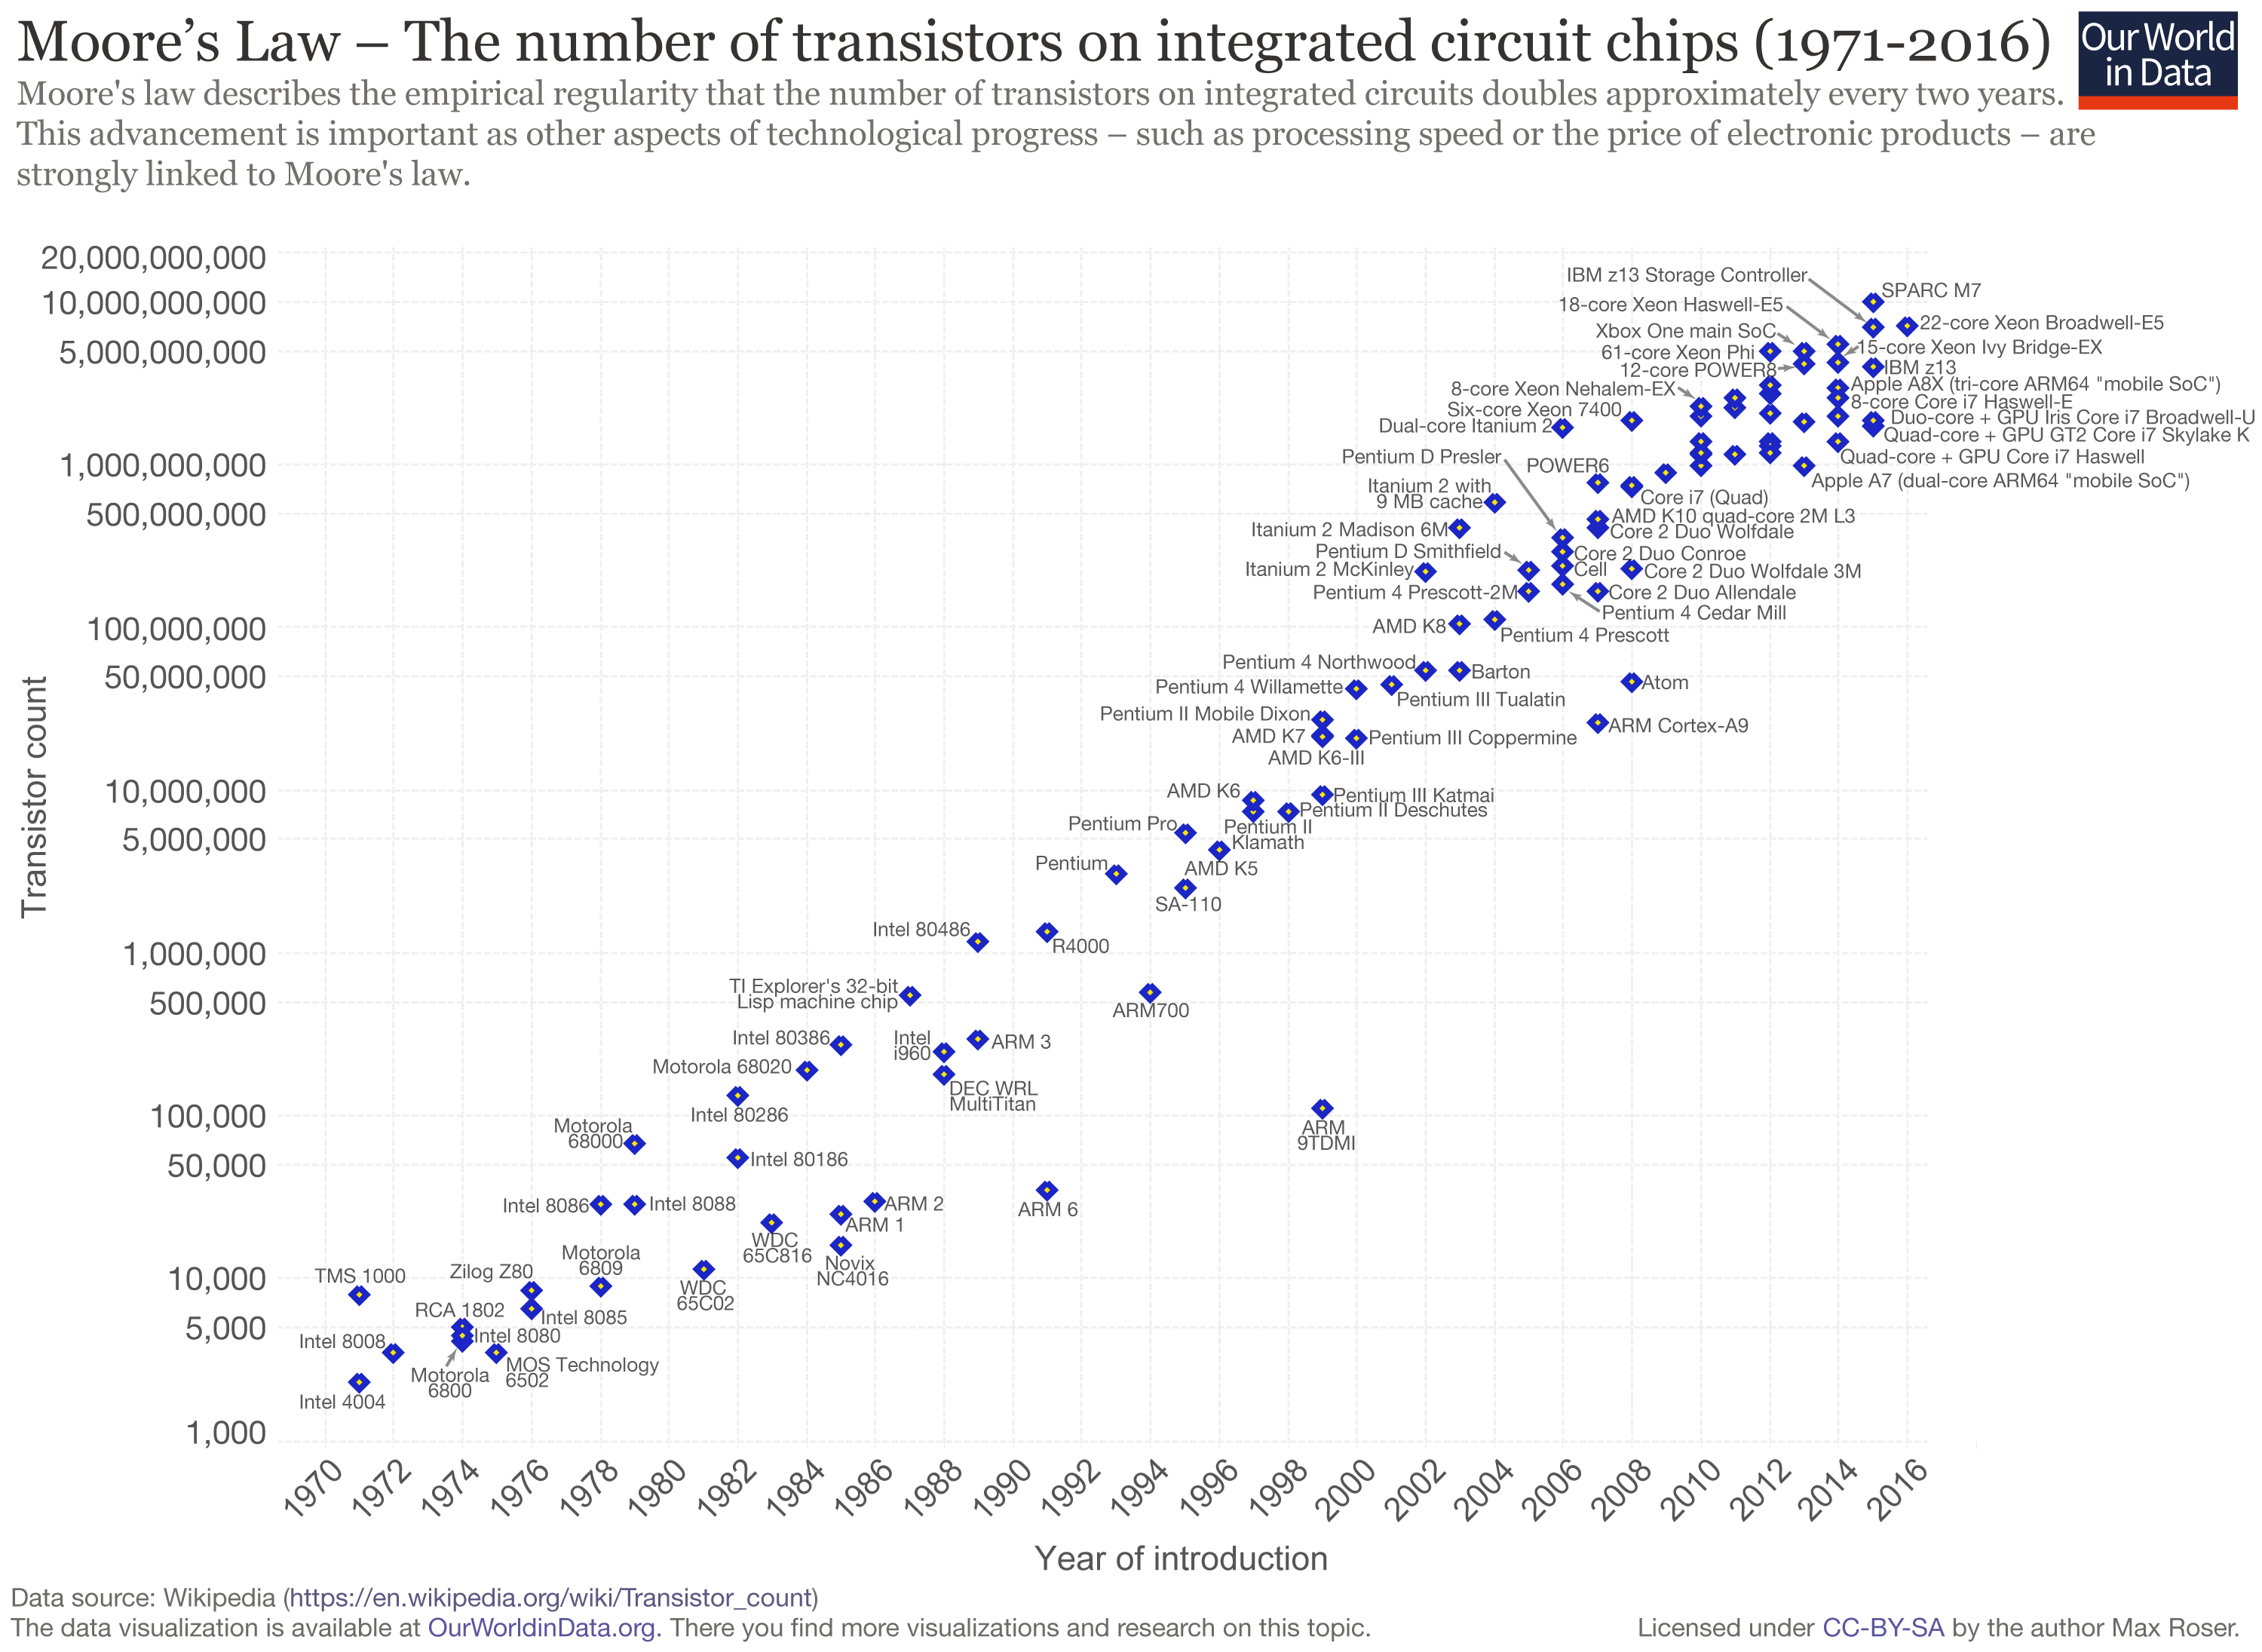
\includegraphics{moorelaw.png}
\caption{The number of transistors throughout the years. We can observe
a recent start of a decline}
\end{figure}

\subsection{The rise of Hardware}\label{the-rise-of-hardware}

Hardware and Software designate here respectively programs that are
executed as code for a general purpose processing unit and programs that
are encoded in the circuits. The dichotomy is not very well defined and
we can think of it as a spectrum. General-purpose computing on graphics
processing units (GPGPU) is in-between. Very efficient when appropriate
and used well. They have benefited from high-investment and many
generation of iterations and hence, for some tasks, can rivalize or even
surpass Hardware.

\begin{figure}
\centering
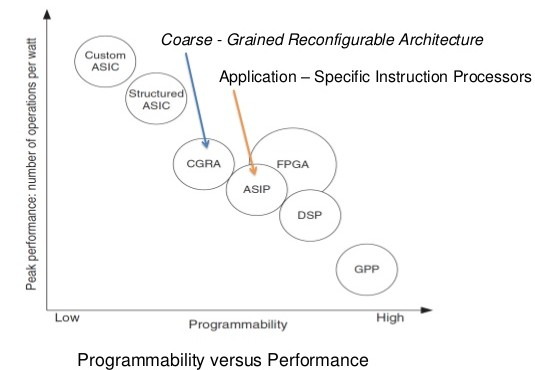
\includegraphics{hwsf.jpg}
\caption{Hardware vs Software}
\end{figure}

Hardware has always been there but application-specific integrated
circuit (ASIC) has prohibitive costs upfront (in the range of \$100M for
a tapeout). Reprogrammable hardware like field-programmable gate array
(FPGA) have only been used marginally and for some specific industry
like high-frequency trading. But now Hardware might be the only solution
(until a computing revolution happen, like quantum computing, but this
is not realist for the near future) to increase performance. But
hardware do not enjoy the same quality of tool, language and integrated
development environment (IDE) as software. This is the motivation behind
Spatial.

\subsection{Hardware as companion
accelerators}\label{hardware-as-companion-accelerators}

In most case, hardware would be inappropriate: running an OS as hardware
would be irrealist. However, as a companion to a central-processing unit
(CPU also called ``the host''), you are able to get the best of both
world. The flexibility of software on a CPU with the speed of hardware.
In this setup, hardware is considered an ``accelerator'' (Hence, the
term ``accelerating hardware''). It accelerates the most demanding
subroutines of the CPU. This companionship is already present in modern
computer desktops under the form of GPUs for \emph{shader} operations
and sound card for complex sound transformation/output.

\subsection{The right metric:
Perf/Watt}\label{the-right-metric-perfwatt}

The right metric for accelerator is performance by energy, as measured
in FLOPS per Watt. This is a fair metric for the comparison of different
hardware because it shows the intrisic value of the architecture. If the
metric was solely performance, then it would suffice to combine multiple
of the same architecture. Perf per dollar is not a good metric either
because you should also account for the cost of energy at runtime.
Hence, Perf/Watt seems like a fair metric to compare architectures.

\subsection{Spatial}\label{spatial}

At the dawn lab, under the lead of
\href{http://arsenalfc.stanford.edu/kunle}{Prof.~Kunle} and his grad
students, is developped a scala DSL
\href{https://github.com/stanford-ppl/spatial-lang}{spatial} and its
compiler to program Hardware in a higher-level, more user-friendly, more
productive language than Verilog. In particular, the control flows are
automatically generated when possible. This should enable software
engineers to unlock the potential of Hardware. A custom CGRA,
Plasticine, has been developped in parralel to Spatial. It leverages
some recurrent patterns, in particular parralel patterns and aims to be
the most efficient reprogrammable architecture for Spatial.

There is a large upfront cost but once at a big enough scale, Plasticine
could be deployed as an accelerator for most demanding server
applications and embedded systems with heavy computing requirements.

\subsection{Embedded systems and
drones}\label{embedded-systems-and-drones}

Embedded systems are limited by the amount of power at disposal from the
battery and might also have size constraints. At the same time,
especially for autonomous vehicles, there is a great need for computing
power.

Thus, developping drone applications with spatial demonstrates the
advantages of the platform. As a matter of fact, the filter that has
been developped was only made possible because it was run on an
accelerating hardware. It would be irrealist to attempt to run it on
more conventional micro-transistors. This is why the family in which
belong the filter developped here, particles filters, being very
computationally expensive, are very seldom used for drones.

\section{Part I: Accelerated optimal sensor fusion algorithm for POSE
estimation of drones: Asynchronous Rao-Blackwellized Particle
filter"}\label{part-i-accelerated-optimal-sensor-fusion-algorithm-for-pose-estimation-of-drones-asynchronous-rao-blackwellized-particle-filter}

POSE is the combination of the position and orientation of an object.
POSE estimation is important for drones. It is a subroutine of SLAM
(Simultaneous localization and mapping) and it is a central part of
motion planning and motion control. More accurate and more reliable POSE
estimation results in more agile, more reactive and safer drones. Drones
are an intellectually stimulating subject but in the near-future they
might also see their usage increase exponentially. In this context,
developping and implementing new filter for POSE estimation is both
important for the field of robotics but also to demonstrate the
importance of hardware acceleration. Indeed, the best and last filter
presented here is only made possible because it can be hardware
accelerated with Spatial. However, the spatial implementation will be
presented in Part III.

Before expanding on the Rao-Blackwellized particle filter, we will
introduce here several other filters for POSE estimation for highly
dynamic objects: Complementary filter, Kalman Filter, Extended Kalman
Filter and finally Rao-Blackwellized Particle filter. The order is from
the most conceptually simple, to the most complex. This order is
justified because complex filters aim to alleviate some of the flaws of
their simpler counterpart. It is important to understand what are those
weakness and how we can alleviate them.

\subsection{Drones and collision
avoidance}\label{drones-and-collision-avoidance}

The original motivation for the development of accelerated POSE
estimation is for the task of collision avoidance by quadcopters. In
particular, a collision avoidance algorithm developped at the
\href{https://asl.stanford.edu/}{ASL lab} and demonstrated here
\href{https://www.youtube.com/watch?v=kdlhfMiWVV0}{(https://youtu.be/kdlhfMiWVV0)}

\begin{figure}
\centering
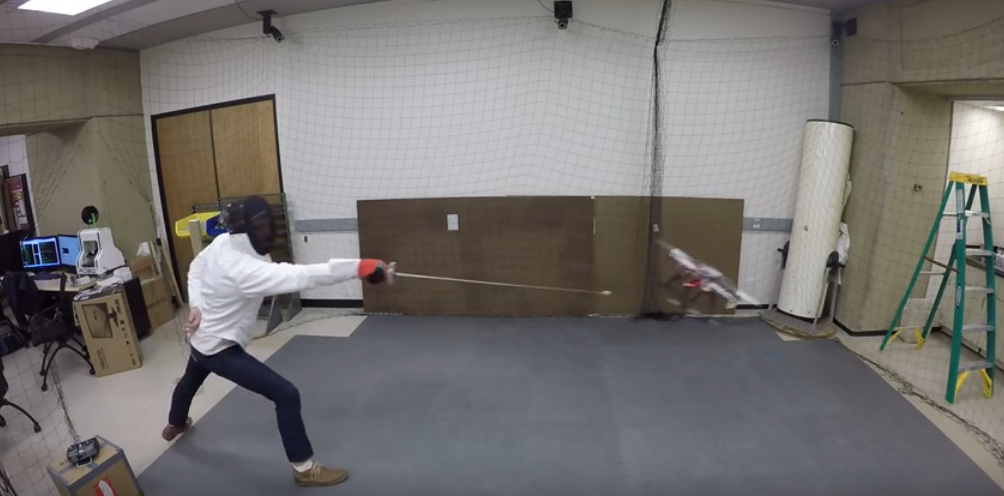
\includegraphics{fencing.png}
\caption{Ross Allen fencing with his drone}
\end{figure}

where the drone avoids the sword attack froms its creator. At first, it
was thought of accelerating the whole algorithm but it was found that
one of the most demanding subroutine was pose estimation. Moreover, it
was wished to increase the processing rate of the filter such that it
could match the input with the fastest sampling rate: its inertial
measurement unit (IMU) containing an accelerometer, a gyroscope and a
magnetometer.

The flamewheel f450 is the typical drone in this category. It is
surprisingly fast and agile. Given the proper command, it can generate
enough thrust to avoid in a very short lapse of time any incoming
object.

\begin{figure}
\centering
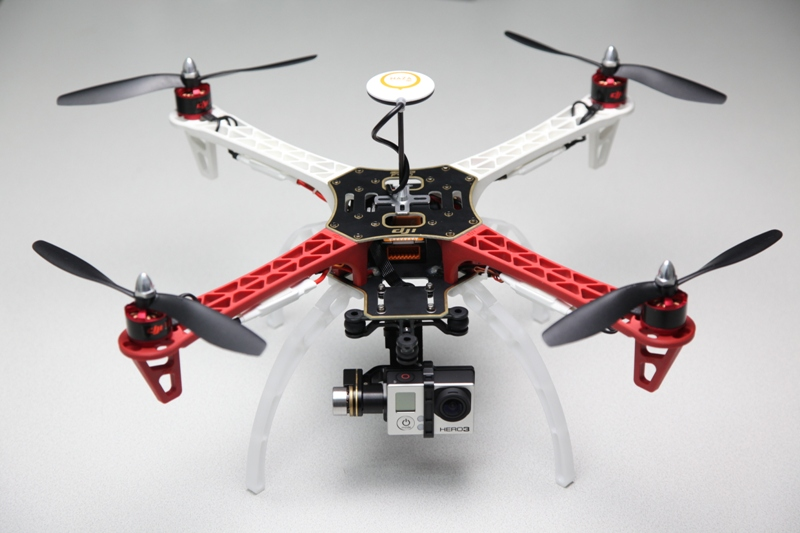
\includegraphics{f450.jpg}
\caption{The Flamewheel f450}
\end{figure}

\subsection{Sensor fusion}\label{sensor-fusion}

Sensor fusion is combining of sensory data or data derived from
disparate sources such that the resulting information has less
uncertainty than would be possible when these sources were used
individually. In the context of drones, it is very useful because it
enables to combine many unprecise sensor measurement to form a more
precise measurement like having precise positionning from 2 less precise
GPS (dual GPS setting). It can also permit to combine sensors with
different sampling rates: typically precise sensors with low sampling
rate and less precise sensors with high sampling rate. Both cases are
gonna be relevant here.

A fundamental explanation why this is possible comes from the central
limit theorem: one sample from a distribution with a low variance is as
good as n sample from a distribution with variance \(n\) times higher.

\[\mathbb{V}(X_i)=\sigma^2 ~~~~~ \mathbb{E}(X_i) = \mu\]
\[\bar{X} = \frac{1}{n}\sum X_i\]
\[\mathbb{V}(\bar{X}) = \frac{\sigma^2}{n}  ~~~~~ \mathbb{E}(\bar{X}) = \mu\]

\subsection{Notes on notation and
conventions}\label{notes-on-notation-and-conventions}

The referential by default is the fixed world frame.

\begin{itemize}
\tightlist
\item
  \(\mathbf{x}\) designates a vector
\item
  \(x_t\) is the random variable of x at time t
\item
  \(x_{t1:t2}\) is the product of the random variable of x between t1
  included and t2 included
\item
  \(x^{(i)}\) designates the random variable x of the arbitrary particle
  i
\item
  \(\hat{x}\) designates an estimated variable
\end{itemize}

\subsection{POSE}\label{pose}

POSE is the task of estimating the position and orientation of an object
through time. It is a subroutine of Software Localization And Mapping
(SLAM). We can formelize the problem as:

At each timestep, find the best expectation of a function of the hidden
variable state (position and orientation), from their initial
distribution and the history of observable random variables (such as
sensor measurements).

\begin{itemize}
\tightlist
\item
  The state \(\mathbf{x}\)
\item
  The function \(g(\mathbf{x})\) such that
  \(g(\mathbf{x}_t) = (\mathbf{p}_t, \mathbf{q}_t)\) where
  \(\mathbf{p}\) is the position and \(\mathbf{q}\) is the attitude as a
  quaternion.
\item
  The observable variable \(\mathbf{y}\) composed of the sensor
  measurements \(\mathbf{z}\) and the control input \(\mathbf{u}\)
\end{itemize}

The algorithm inputs are:

\begin{itemize}
\tightlist
\item
  control inputs \(\mathbf{u}_t\) (the commands sent to the flight
  controller)
\item
  sensor measurements \(\mathbf{z}_t\) coming from different sensors
  with different sampling rate
\item
  information about the sensors (sensor measurements biases and matrix
  of covariance)
\end{itemize}

\subsection{Data generation}\label{data-generation}

\textbf{TODO}

\subsection{Quaternion}\label{quaternion}

Quaternions are extensions of complex numbers but with 3 imaginary
parts. Unit quaternions can be used to represent orientation, also
referred to as attitude. Quaternions algebra make rotation composition
simple and quaternions avoid the issue of gimbal lock. In all filters
presented, they will be used to represent the attitude.

\[\mathbf{q} = (q.r, q.i, q.j, q.k)^t = (q.r, \boldsymbol{\varrho})^T\]

Quaternion rotations composition is: \(q_2 q_1\) which results in
\(q_1\) being rotated by the rotation represented by \(q_2\). From this,
we can deduce that angular velocity integrated over time is simply
\(q^t\) if \(q\) is the local quaternion rotation by unit of time.

Rotation of a vector by a quaternion is done by: \(q v q^*\) where \(q\)
is the quaternion representing the rotation, \(q^*\) its conjugate and
\(v\) the vector to be rotated.

The distance of between two quaternions, useful as an error metric is
defined by the squared Frobenius norms of attitude matrix differences
{[}\protect\hyperlink{ref-markley_averaging_2007}{1}{]}.

\[\| A(\mathbf{q}_1) - A(\mathbf{q}_2) \|^2_F = 6 - 2 Tr [ A(\mathbf{q}_1)A^t(\mathbf{q}_2) ]\]

where

\[A(\mathbf{q}) = (q.r^2 - \| \boldsymbol{\varrho} \|^2) I_{3 \times 3} + 2\boldsymbol{\varrho} \boldsymbol{\varrho}^T - 2q.r[\boldsymbol{\varrho} \times]\]

\[[\boldsymbol{\varrho} \times] = \left( \begin{array}{ccc}
0 & -q.k & q.j \\
q.k & 0 & -q.i \\
-q.j & q.i & 0 \\
\end{array} \right)\]

\subsection{Helper functions and
matrices}\label{helper-functions-and-matrices}

We introduce some helper matrices.

\begin{itemize}
\tightlist
\item
  \(\mathbf{R}_{b2f}\{\mathbf{q}\}\) is the body to fixed vector
  rotation matrix. It transforms vector in the body frame to the fixed
  world frame. It takes as parameter the attitude \(\mathbf{q}\).
\item
  \(\mathbf{R}_{f2b}\{\mathbf{q}\}\) is its inverse matrix (from fixed
  to body).
\item
  \(\mathbf{T}_{2a} = (0, 0, 1/m)^T\) is the scaling from thrust to
  acceleration (by dividing by the weight of the drone:
  \(\mathbf{F} = m\mathbf{a} \Rightarrow \mathbf{a} = \mathbf{F}/m)\)
  and then multiplying by a unit vector \((0, 0, 1)\)
\item
  \[R2Q(\boldsymbol{\theta}) = (\cos(\| \boldsymbol{\theta} \| / 2), \sin(\| \boldsymbol{\theta} \| / 2) \frac{\boldsymbol{\theta}}{\| \boldsymbol{\theta} \|} )\]
  is a function that convert from a local \emph{rotation vector}
  \(\boldsymbol{\theta}\) to a local quaternion rotation. The definition
  of this function come from converting \(\boldsymbol{\theta}\) to a
  body-axis angle, and then to a quaternion.
\item
  \[Q2R(\mathbf{q}) = (q.i*s, q.j*s, q.k*s) \] is its inverse function
  where \(n = \arccos(q.w)*2\) and \(s = n/\sin(n/2)\)
\item
  \(\Delta t\) is the lapse of time between t and the next tick (t+1)
\end{itemize}

\subsection{Model}\label{model}

The drone is assumed to have rigid-body physics. It is submitted to the
gravity and its own inertia. A rigid body is a solid body in which
deformation is zero or so small it can be neglected. The distance
between any two given points on a rigid body remains constant in time
regardless of external forces exerted on it. This enable to summarise
the forces from the rotor as a thrust oriented in the direction normal
to the plane formed by the 4 rotosrs, and an angular velocity.

Those variables are sufficient to describe the evolution of our drone
with rigid-body physics:

\begin{itemize}
\tightlist
\item
  \(\mathbf{a}\) the total acceleration in the fixed world frame
\item
  \(\mathbf{v}\) the velocity in the fixed world frame
\item
  \(\mathbf{p}\) the position in the fixed world frame
\item
  \(\boldsymbol{\omega}\) the angular velocity
\item
  \(\mathbf{q}\) the attitude in the fixed world frame
\end{itemize}

\subsection{Sensors}\label{sensors}

The sensors at disposition are:

\begin{itemize}
\item
  \textbf{Accelerometer}: It generates \(\mathbf{a_A}\) a measurement of
  the total acceleration in the body frame referrential the drone is
  submitted to at a \textbf{high} sampling rate. If the object is
  submitted to no acceleration then the accelerometer measure the
  earth's gravity field from. From that information, it could be
  possible to retrieve the attitude. Unfortunately, we are in a highly
  dynamic setting. Thus, it is possible when we can substract the
  drone's acceleration from the thrust to the total acceleration. This
  would require to know exactly the force exerced by the rotors at each
  instant. In this work, we assume that doing that separation, while
  being theoretically possible, is too impractical. The measurements
  model is:
  \[\mathbf{a_A}(t) = \mathbf{R}_{f2b}\{\mathbf{q}(t)\}\mathbf{a}(t) + \mathbf{a_A}^\epsilon\]
  where the covariance matrix of the noise of the accelerometer is
  \({\mathbf{R}_{\mathbf{a_A}}}_{3 \times 3}\) and
  \[\mathbf{a_A}^\epsilon \sim \mathcal{N}(\mathbf{0}, \mathbf{R}_{\mathbf{a_A}})\].
\item
  \textbf{Gyroscope}:It generates \(\mathbf{\boldsymbol{\omega}_G}\) a
  measurement of the angular velocity in the body frame of the drone at
  the last timestep at a \textbf{high} sampling rate. The measurement
  model is:
  \[\mathbf{\boldsymbol{\omega}_G}(t) = \boldsymbol{\omega} + \mathbf{\boldsymbol{\omega}_G}^\epsilon\]
  where the covariance matrix of the noise of the accelerometer is
  \({\mathbf{R}_{\mathbf{\boldsymbol{\omega}_G}}}_{3 \times 3}\) and
  \[\mathbf{\boldsymbol{\omega}_G}^\epsilon_t \sim \mathcal{N}(\mathbf{0}, \mathbf{R}_{\mathbf{\boldsymbol{\omega}_G}})\].
\item
  \textbf{Position}: It generates \(\mathbf{p_V}\) a measurement of the
  current positionat a \textbf{low} sampling rate. This is usually
  provided by a \textbf{Vicon} (for indoor), \textbf{GPS}, a
  \textbf{Tango} or any other position sensor. The measurement model is:
  \[\mathbf{p_V}(t) = \mathbf{p}(t) + \mathbf{p_V}^\epsilon\] where the
  covariance matrix of the noise of the position is
  \({\mathbf{R}_{\mathbf{p_V}}}_{3 \times 3}\) and
  \[\mathbf{p_V}^\epsilon \sim \mathcal{N}(\mathbf{0}, \mathbf{R}_{\mathbf{p_V}})\].
\item
  \textbf{Attitude}: It generates \(\mathbf{q_V}\) a measurement of the
  current attitute. This is usually provided in addition to the position
  by a \textbf{Vicon} or a \textbf{Tango} at a \textbf{low} sampling
  rate or the \textbf{Magnemoter} at a \textbf{high} sampling rate if
  the environment permit it (no high magnetic interference nearby like
  iron contamination). The magnetometer retrieve the attitude by
  assuming that the sensed magnetic field corresponds to the earth's
  magnetic field. The measurement model is:
  \[\mathbf{q_V}(t) = \mathbf{q}(t)*R2Q(\mathbf{q_V}^\epsilon)\] where
  the \(3 \times 3\) covariance matrix of the noise of the attitude in
  radian before being converted by \(R2Q\) is
  \({\mathbf{R}_{\mathbf{q_V}}}_{3 \times 3}\) and
  \[\mathbf{q_V}^\epsilon \sim \mathcal{N}(\mathbf{0}, \mathbf{R}_{\mathbf{q_V}})\].
\item
  \textbf{Optical Flow}: A camera that keeps track of the movement by
  comparing the difference of the position of some reference points. By
  using a companion distance sensor, it is able to retrieve the
  difference between the two perspective and thus the change in angle
  and position.
  \[\mathbf{dq_O}(t) = (\mathbf{q}(t-k)\mathbf{q}(t))*R2Q(\mathbf{dq_O}^\epsilon)\]
  \[\mathbf{dp_O}(t) = (\mathbf{p}(t) - \mathbf{p}(t-k)) + \mathbf{dp_O}^\epsilon\]
\end{itemize}

where the \(3 \times 3\) covariance matrix of the noise of the attitude
variation in radian before being converted by \(R2Q\) is
\({\mathbf{R}_{\mathbf{dq_O}}}_{3 \times 3}\) and
\[\mathbf{dq_O}^\epsilon \sim \mathcal{N}(\mathbf{0}, \mathbf{R}_{\mathbf{dq_O}})\]
and the position variation covariance matrix
\({\mathbf{R}_{\mathbf{dp_O}}}_{3 \times 3}\) and
\[\mathbf{dp_O}^\epsilon \sim \mathcal{N}(\mathbf{0}, \mathbf{R}_{\mathbf{dp_O}})\].

\begin{figure}
\centering
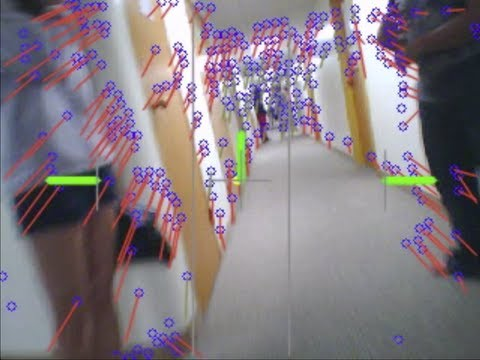
\includegraphics{opflow.jpg}
\caption{Optical flow from a moving drone}
\end{figure}

The notable difference with the position or attitude sensor is that the
optical flow sensor, like the IMU, only captures time variation, not
absolute values.

\begin{itemize}
\tightlist
\item
  \textbf{Altimeter}: An altimeter is a sensor that measure the altitude
  of the drone. For instance a LIDAR measure the time for the laser wave
  to reflect on a surface that is assumed to be the ground. A smart
  strategy is to only use the altimeter is oriented with a low angle to
  the earth, else you also have to account that angle in the estimation
  of the altitude.
  \[z_A(t) = \sin(\text{pitch}(\mathbf{q(t)}))(\mathbf{p}(t).z + z_A^\epsilon)\]
  \({R_{z_A}}_{3 \times 3}\) and
  \[z_A^\epsilon \sim \mathcal{N}(0, R_{z_A})\]
\end{itemize}

\begin{figure}
\centering
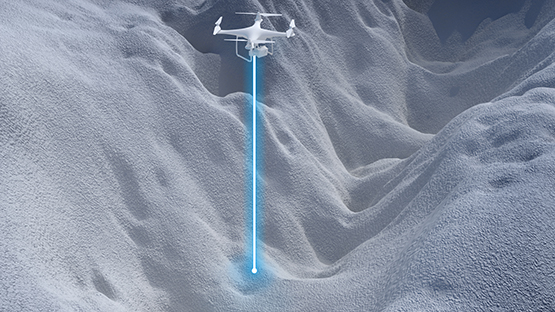
\includegraphics{altimeter.jpg}
\caption{Rendering of the LIDAR laser of an altimeter}
\end{figure}

Some sensors are more relevant indoor and some others outdoor:

\begin{itemize}
\tightlist
\item
  \textbf{Indoor}: The sensors available indoor are the accelerometer,
  the gyroscope and the \textbf{Vicon}. The Vicon is a system composed
  of many sensors around a room that is able to track very accurately
  the position and orientation a mobile object. One issue with relying
  solely on the \textbf{Vicon} is that the sampling rate is low.
\end{itemize}

\begin{figure}
\centering
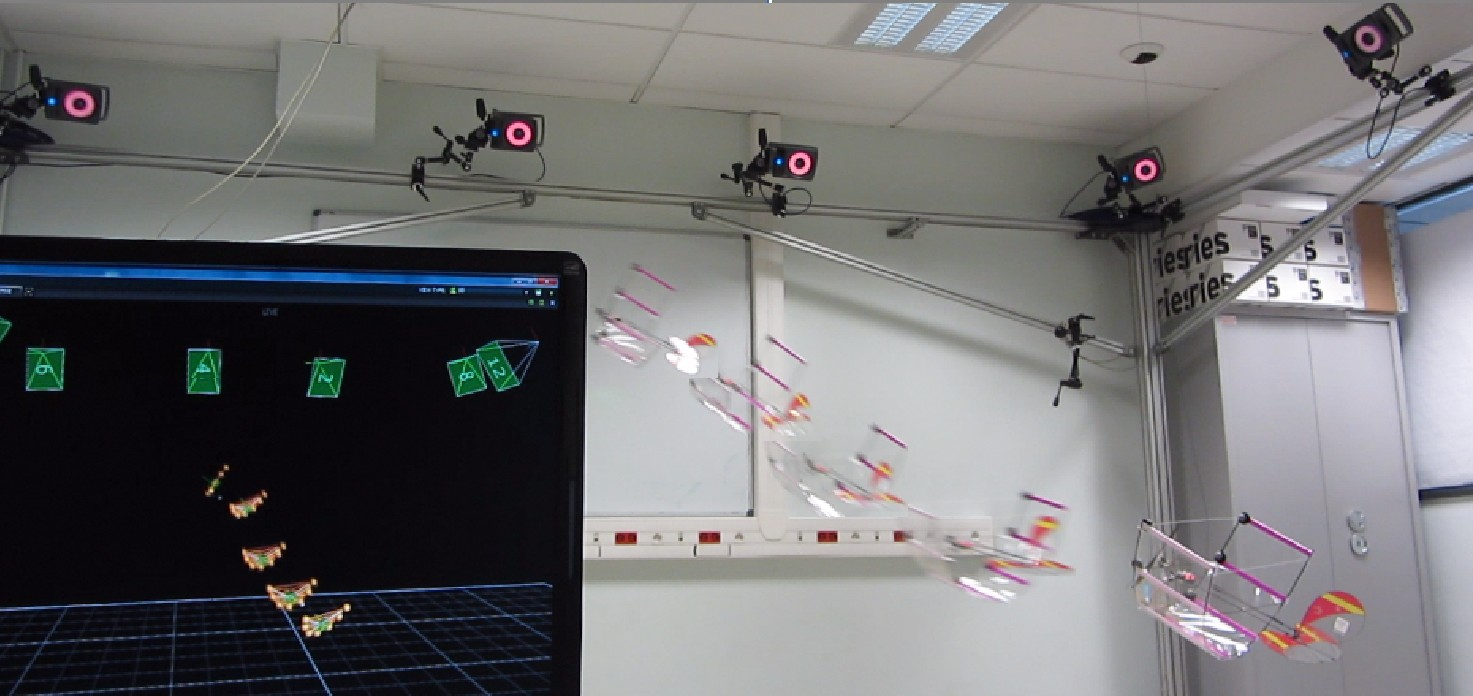
\includegraphics{vicon.jpg}
\caption{A Vicon setup}
\end{figure}

\begin{itemize}
\tightlist
\item
  \textbf{Outdoor}: The sensors available outdoor are the accelerometer,
  the gyroscope, the magnetometer, two GPS, an optical flow and an
  altimeter.
\end{itemize}

We assume that since the biases of the sensor could be known prior to
the flight, the sensor have been calibrated and output measurements with
no bias. Some filters like the
\href{https://dev.px4.io/en/tutorials/tuning_the_ecl_ekf.html}{ekf2} of
the px4 flight stack keep track of the sensor biases but this is a state
augmentation that was not deemed worthwhile.

\subsubsection{Control inputs}\label{control-inputs}

Observations from the control input are not strictly speaking
measurements but input of the state-transition model. The IMU is a
sensor, thus stricly speaking, its measurements are not control inputs.
However, in the literature, it is standard to use its measurements as
control inputs. One of the advantage is that the accelerometer measures
acceleration and angular velocity, raw values close from the input we
need in our state-transition. If we used a transformation of the thrust
sent as command to the rotors, we would have to account for the rotors
unprecision, the wind and other disturbances. Another advantage is that
since the IMU has very high sampling rate, we can update very frequently
the state with new transitions. The drawback is that the accelerometer
is noisy. Fortunately, we can take into account the noise as a process
model noise.

The control inputs at disposition are:

\begin{itemize}
\tightlist
\item
  \textbf{Acceleration}: \(\mathbf{a_A}_t\) from the acceloremeter
\item
  \textbf{Angular velocity}: \(\mathbf{\boldsymbol{\omega}_G}_t\) from
  the gyroscope.
\end{itemize}

\hypertarget{model-dynamic}{\subsubsection{Model
dynamic}\label{model-dynamic}}

\begin{itemize}
\tightlist
\item
  \(\mathbf{a}(t+1) = \mathbf{R}_{b2f}\{\mathbf{q}(t+1)\}(\mathbf{a_A}_t + \mathbf{a_A}^\epsilon_t)\)
  where
  \(\mathbf{a}^\epsilon_t \sim \mathcal{N}(\mathbf{0}, \mathbf{Q}_{\mathbf{a}_t })\)
\item
  \(\mathbf{v}(t+1) = \mathbf{v}(t) + \Delta t \mathbf{a}(t) + \mathbf{v}^\epsilon_t\)
  where
  \(\mathbf{v}^\epsilon_t \sim \mathcal{N}(\mathbf{0}, \mathbf{Q}_{\mathbf{v}_t })\)
\item
  \(\mathbf{p}(t+1) = \mathbf{p}(t) + \Delta t \mathbf{v}(t) + \mathbf{p}^\epsilon_t\)
  where
  \(\mathbf{p}^\epsilon_t \sim \mathcal{N}(\mathbf{0}, \mathbf{Q}_{\mathbf{p}_t })\)
\item
  \(\boldsymbol{\omega}(t+1) = \mathbf{\boldsymbol{\omega}_G}_t + \mathbf{\boldsymbol{\omega}_G}^\epsilon_t\)
  where
  \(\mathbf{p}^\epsilon_t \sim \mathcal{N}(\mathbf{0}, \mathbf{Q}_{\mathbf{\boldsymbol{\omega}_G}_t })\)
\item
  \(\mathbf{q}(t+1) = \mathbf{q}(t)*R2Q(\Delta t \boldsymbol{ \omega(t) })\)
\end{itemize}

Note that in our model, \(\mathbf{q}(t+1)\) must be known. Fortunately,
as we will see later, our Rao-Blackwellized Particle Filter is
conditionned under the attitude so it is known.

\subsection{State}\label{state}

The time series of the variables of our dynamic model constitute a
hidden markov chain. Indeed, the model is ``memoryless'' and depends
only on the current state and a sampled transition.

States contain variables that enable us to keep track of some of those
hidden variables which is our ultimate goal (for POSE \(\mathbf{p}\) and
\(\mathbf{q}\)). States at time \(t\) are denoted by \(\mathbf{x}_t\).
Different filters require different state variables depending on their
structure and assumptions.

\subsection{Observation}\label{observation}

Observations are revealed variables conditionned under the variables of
our dynamic model. Our ultimate goal is to deduce the states from the
observations.

Observations contain the control input \(\mathbf{u}\) and the
measurements \(\mathbf{z}\).

\[\mathbf{y}_t = (\mathbf{z}_t, \mathbf{u}_t)^T = (\mathbf{p_V}_t, \mathbf{q_V}_t), ({t_C}_t, \mathbf{\boldsymbol{\omega}_C}_t))^T\]

\subsection{Filtering and smoothing}\label{filtering-and-smoothing}

\textbf{Smoothing} is the statistical task of finding the expectation of
the state variable from the past history of observations and multiple
observation variables ahead

\[\mathbb{E}[g(\mathbf{x}_{0:t}) | \mathbf{y}_{1:t+k}]\]

Which expand to,

\[\mathbb{E}[(\mathbf{p}_{0:t}, \mathbf{q}_{0:t}) | (\mathbf{z}_{1:t+k}, \mathbf{u}_{1:t+k})]\]

\(k\) is a contant and the first observation is \(y_1\)

\textbf{Filtering} is a kind of smoothing where you only have at
disposal the current observation variable (\(k=0\))

\subsection{Complementary Filter}\label{complementary-filter}

The complementary filter is the simplest of all filter and very common
to retrieve the attitude because of its low computational complexity.
The gyroscope and accelerometer both provide a measurement that can help
us to estimate the attitude. The gyroscope indeed gives us a noisy
measurement of the angular velocity from which we can retrieve the new
attitude from the past one by time integration:
\(\mathbf{q}_t = \mathbf{q}_{t-1}*R2Q(\Delta t \mathbf{\omega})\).

This is commonly called ``Dead reckoning''\footnote{The etymology for
  ``Dead reckoning'' comes from the mariners of the XVIIth century that
  used to calculate the position of the vessel with log book. The
  interpretation of ``dead'' is subject to debate. Some argue that it is
  a mispelling of ``ded'' as in ``deduced''. Others argue that it should
  be read by its old meaning: \emph{absolute}.} and is prone to
accumulation error, referred as drift. Indeed, like brownian motions,
even if the process is unbiased, the variance grows with time. Reducing
the noise cannot solve the issue entirely: even with extremely precise
instruments, you are subject to floating point errors.

Fortunately, even though the accelerometer gives us a highly noisy
(vibrations, wind, etc \ldots{} ) measurement of the orientation, it is
not subject to drift because it does not rely on accumulation. Indeed,
if not subject to other accelerations, the accelerometer measures the
gravity field orientation. Since this field is oriented toward earth, it
is possible to retrieve the current rotation from that field and by
extension the attitude. However, in the case of a drone, it is subject
to continuous and signifiant acceleration and vibration. Hence, the
assumption that we retrieve the gravity field directly is wrong.
Nevertheless, We could solve this by substracting the acceleration
deduced from the thrust control input. It is unpractical so this
approach is not pursued in this work, but understanding this filter is
still useful.

The idea of the filter itself is to combine the precise ``short-term''
measurements of the gyroscope subject to drift with the ``long-term''
measurements of the accelerometer.

\subsubsection{State}\label{state-1}

This filter is very simple and it is only needed to store as a state the
last estimated attitude along with its timestamp (to calculate
\(\Delta t\)). \[\mathbf{x}_t = \mathbf{q}_t\]
\[\hat{\mathbf{q}}_{t+1} = \alpha (\hat{\mathbf{q}}_t + \Delta t \mathbf{\omega}_t) + (1 - \alpha) {\mathbf{q_A}}_{t+1}\]
\(\alpha \in [0, 1]\). Usually, \(\alpha\) is set to a high-value like
\(0.98\). It is very intuitive to see why this should approximately
``work'', the data from the accelerometer continuously correct the drift
from the gyroscope.

\begin{figure}
\centering
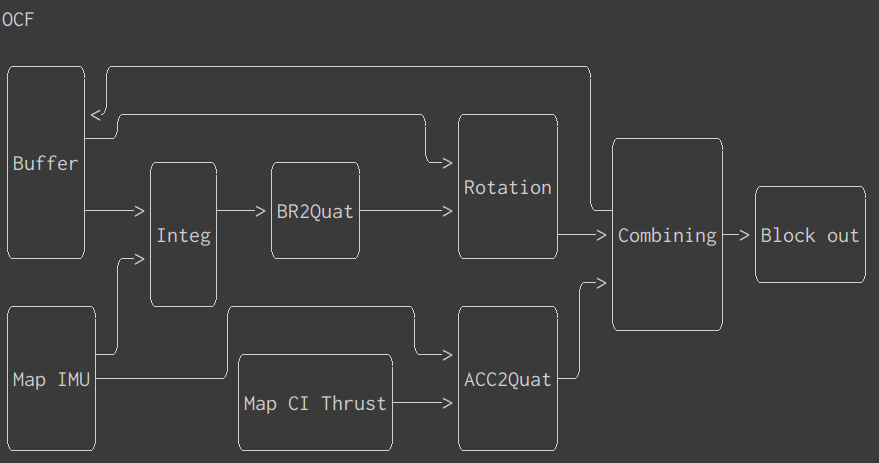
\includegraphics{ocf.png}
\caption{CF Graph generated by scala-flow}
\end{figure}

Figure 9 is the plot of the distance from the true quaternion after 15s
of an arbitrary trajectory when \(\alpha = 1.0\) meaning that the
accelerometer does not correct the drift.

\begin{figure}
\centering
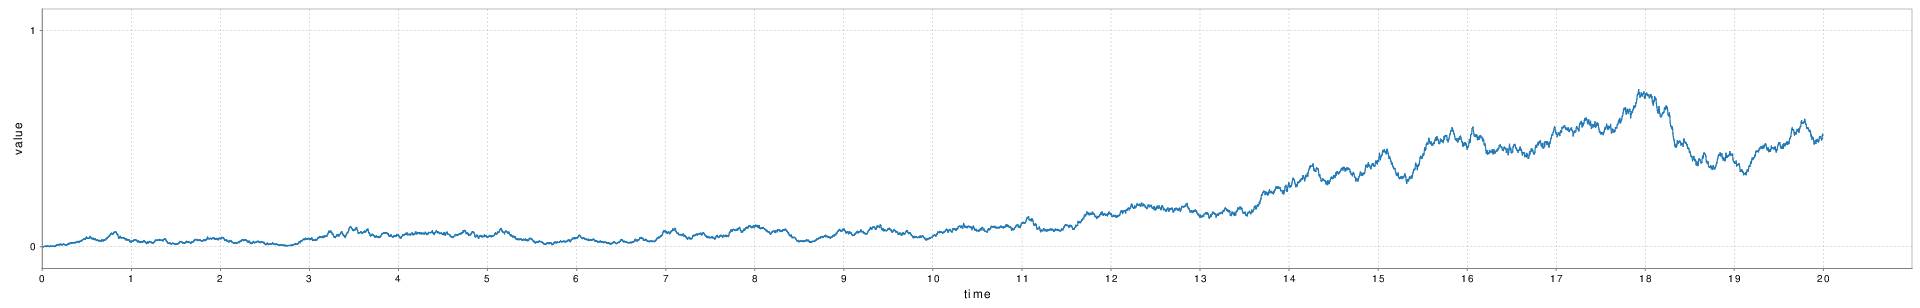
\includegraphics{cf100.png}
\caption{CF with alpha = 1.0}
\end{figure}

Figure 10 is that same trajectory with \(\alpha = 0.98\).

\begin{figure}
\centering
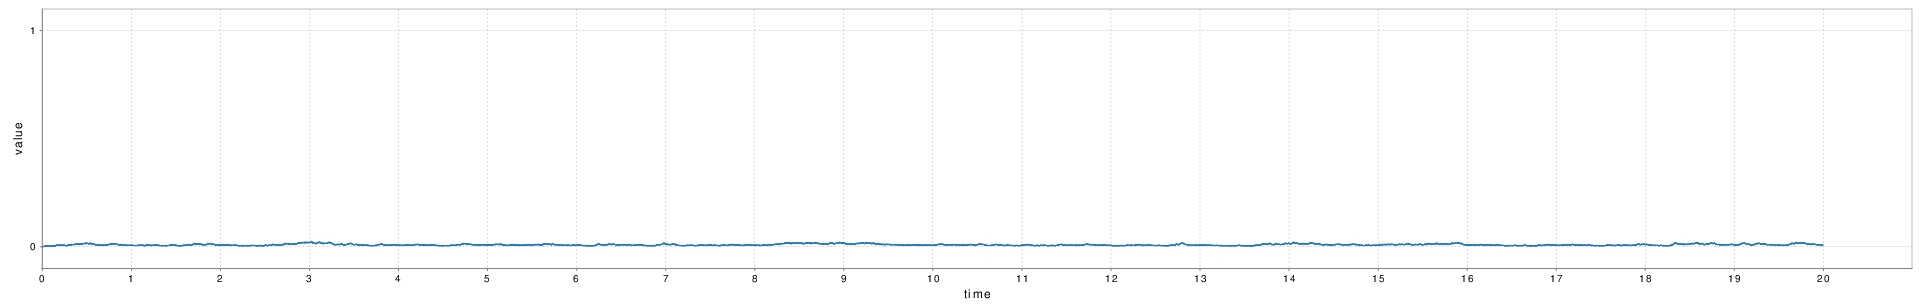
\includegraphics{cf098.png}
\caption{CF with alpha = 0.98}
\end{figure}

\subsection{Asynchronous Augmented Complementary
Filter}\label{asynchronous-augmented-complementary-filter}

As explained previously, in this highly-dynamic setting, combining the
gyroscope and the accelerometer to retrieve the attitude is not
satisfactory. However, we can reuse the intuition from the complementary
filter, which is to combine precise but drifting short-term measurement
to other measurements that do not suffer from drift. This enable a
simple and computionally inexpensive novel filter that we will be able
to use later as a baseline. In this case, the short-term measurements
are the acceleration and angular velocity from the IMU, and the non
drifting measurements come from the Vicon.

We will also add the property that the data from the sensors are
asynchronous. This is a consequence of the sensors having different
sampling rate.

\begin{itemize}
\item
  \textbf{IMU} update
  \[\mathbf{v}_t = \mathbf{v}_{t-1} + \Delta t_v \mathbf{a_A}_t\]
  \[\boldsymbol{\omega}_t = \boldsymbol{\mathbf{\omega_G}}_t\]
  \[\mathbf{p}_t = \mathbf{p}_{t-1} + \Delta t \mathbf{v}_{t-1}\]
  \[\mathbf{q}_t = \mathbf{q}_{t-1}R2Q(\Delta t \boldsymbol{\omega}_{t-1})\]
\item
  \textbf{Vicon} update
  \[\mathbf{p}_t = \alpha \mathbf{p_V} + (1 - \alpha) (\mathbf{p}_{t-1} + \Delta t \mathbf{v}_{t-1})\]
  \[\mathbf{q}_t = \alpha \mathbf{q_V} + (1 - \alpha) (\mathbf{q}_{t-1}R2Q(\Delta t \boldsymbol{\omega}_{t-1}))\]
\end{itemize}

\subsubsection{State}\label{state-2}

The state has to be more complex because the filter estimate now both
the position and the attitude. Furthermore, because of asynchronousity,
we have to store the last angular velocity, the last linear velocity,
and the last time the linear velocity has been updated (to retrieve
\(\Delta t_v = t - t_a\) where \(t_a\) is the last time we had an update
from the accelerometer).

\[\mathbf{x}_t = (\mathbf{p}_t, \mathbf{q}_t, \boldsymbol{\omega}_t, \mathbf{a}_t, t_a)\]

\begin{figure}
\centering
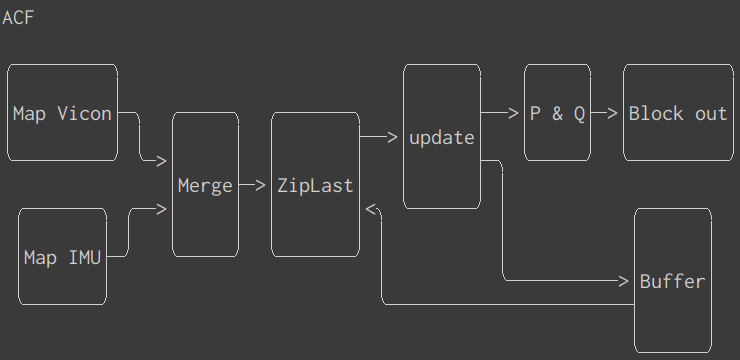
\includegraphics{acf.png}
\caption{AACF Graph generated by scala-flow}
\end{figure}

\subsection{Kalman Filter}\label{kalman-filter}

\subsubsection{Bayesian inference}\label{bayesian-inference}

Bayesian inference is a method of statistical inference in which Bayes'
theorem is used to update the probability for a hypothesis as more
evidence or information becomes available. In this Bayes setting, the
prior is the estimated distribution of the previous state at time
\(t-1\), the likelihood correspond to the likelihood of getting the new
data from the sensor given the prior and finally, the posterior is the
updated estimated distribution.

\subsubsection{Model}\label{model-1}

The kalman filter requires that both the model process and the
measurement process are \textbf{linear gaussian}. Linear gaussian
processes are of the form:
\[\mathbf{x}_t = f(\mathbf{x}_{t-1}) + \mathbf{w}_t\] where \(f\) is a
linear function and \(\mathbf{w}_t\) a gaussian process: it is sampled
from an arbitrary gaussian distribution.

The Kalman filter is a direct application of bayesian inference. It
combines the prediction of the distribution given the estimated prior
state and the state-transition model.

\[\mathbf{x}_t = \mathbf{F}_t \mathbf{x}_{t-1} + \mathbf{B}_t \mathbf{u}_t + \mathbf{w}_t \]

\begin{itemize}
\tightlist
\item
  \(\mathbf{x}_t\) the state
\item
  \(\mathbf{F}_t\) the state transition model
\item
  \(\mathbf{B}_t\) the control-input model
\item
  \(\mathbf{u}_t\) the control vector
\item
  \(\mathbf{w}_t\) process noise drawn from
  \(\mathbf{w}_t \sim N(0, \mathbf{Q}_k)\)
\end{itemize}

and the estimated distribution given the data coming from the sensors.

\[\mathbf{y}_t = \mathbf{H}_t \mathbf{x}_{t}  + \mathbf{v}_t \]

\begin{itemize}
\tightlist
\item
  \(\mathbf{y}_t\) measurements
\item
  \(\mathbf{H}_t\) the state to measurement matrix
\item
  \(\mathbf{w}_t\) measurement noise drawn from
  \(\mathbf{w}_t \sim N(0, \mathbf{R}_k)\)
\end{itemize}

Because, both the model process and the sensor process are assumed to be
linear gaussian, we can combine them into a gaussian distribution.
Indeed, the product of two gaussians is gaussian.

\[P(\mathbf{x}_{t}) \propto P(\mathbf{x}^{-}_{t}|\mathbf{x}_{t-1}) \cdot P(\mathbf{x}_t | \mathbf{y}_t )\]
\[\mathcal{N}(\mathbf{x}_{t}) \propto \mathcal{N}(\mathbf{x}^{-}_{t}|\mathbf{x}_{t-1}) \cdot \mathcal{N}(\mathbf{x}_t | \mathbf{y}_t )\]

where \(\mathbf{x}^{-}_{t}\) is the predicted state from the previous
state and the state-transition model.

The kalman filter keep track of the parameters of that gaussian: the
mean state and the covariance of the state which represent the
uncertainty about our last prediction. The mean of that distribution is
also the best current state estimation of the filter.

By keeping track of the uncertainty, we can optimally combine the
normals by knowing what importance to give to the difference between the
expected sensor data and the actual sensor data. That factor is the
Kalman gain.

\begin{itemize}
\tightlist
\item
  \textbf{predict}:

  \begin{itemize}
  \tightlist
  \item
    predicted \textbf{state}:
    \(\hat{\mathbf{x}}^{-}_t = \mathbf{F}_t \mathbf{x}_{t-1} + \mathbf{B}_t \mathbf{u}_t\)
  \item
    predicted \textbf{covariance}:
    \(\mathbf{\Sigma}^{-}_t = \mathbf{F}_{t-1} \mathbf{\Sigma}^{-}_{t-1} \mathbf{F}_{t-1}^T + \mathbf{Q}_t\)
  \end{itemize}
\item
  \textbf{update}:

  \begin{itemize}
  \tightlist
  \item
    predicted \textbf{measurements}:
    \(\hat{\mathbf{z}} = \mathbf{H}_t \hat{\mathbf{x}}^{-}_t\)
  \item
    \textbf{innovation}: \((\mathbf{z}_t - \hat{\mathbf{z}})\)\\
  \item
    \textbf{innovation covariance}:
    \(\mathbf{S} = \mathbf{H}_t \mathbf{\Sigma}^{-}_t \mathbf{H}_t^T + \mathbf{R}_t\)\\
  \item
    optimal \textbf{kalman gain}:
    \(\mathbf{K} = \mathbf{\Sigma}^{-}_t \mathbf{H}_t^T \mathbf{S}^{-1}\)
  \item
    updated \textbf{state}:
    \(\mathbf{\Sigma}_t = \mathbf{\Sigma}^-_t + \mathbf{K} \mathbf{S} \mathbf{K}^T\)
  \item
    updated \textbf{covariance}:
    \(\hat{\mathbf{x}}_t = \hat{\mathbf{x}}^{-}_t + \mathbf{K}(\mathbf{z}_t - \hat{\mathbf{z}})\)
  \end{itemize}
\end{itemize}

\subsection{Asynchronous Kalman
Filter}\label{asynchronous-kalman-filter}

It is not necessary to apply the full kalman update at each measurement.
Indeed, \(\mathbf{H}\) can be sliced to correspond to the measurements
currently available.

To be truly asynchronous, you also have to account for the different
sampling rates. There is two cases :

\begin{itemize}
\tightlist
\item
  The required data for the update step (the control inputs) can arrive
  multiple time before any of the data of the update step (the
  measurements) occur.
\item
  Inversely, it is possible that the measurements occur at a higher
  sampling rate than the control inputs.
\end{itemize}

The strategy chosen here is as follow:

\begin{enumerate}
\def\labelenumi{\arabic{enumi}.}
\tightlist
\item
  Multiple prediction steps without any update step may happen without
  making the algorithm inconsistent.
\item
  An update is \textbf{always} immediatly preceded by a prediction step.
  This is a consequence of the requirement that the innovation must
  measure the difference between the predicted measurement from the
  state at the exact current time and the measurements. Thus, if the
  measurements are not synchronised with the control inputs, use the
  most likely control input for the prediction step, which might result
  in simply repeating them. Repeating the last control input was the
  method used for the accelerometer and the gyroscope data as control
  input.
\end{enumerate}

\subsection{Extended Kalman Filters}\label{extended-kalman-filters}

In the previous section, we have shown that the Kalman Filter is only
applicable when both the process model and the measurement model are
linear gaussian process. This has two aspects:

\begin{itemize}
\tightlist
\item
  The noise of the measurements and of the state-transition must be
  gaussian
\item
  The state-transition function and the measurement to state function
  must be linear.
\end{itemize}

Furthermore, it is provable that kalman filters are optimal linear
filters.

However, in our context, one component of the state, the attitude, is
intrisically non-linear. Indeed, rotations and attitudes belong to
\(SO(3)\) which is not a vector space. Therefore, we cannot use
\emph{vanilla} kalman filters. The filters that we present thereafter
relax those requirements.

One example of such extension is the extended kalman filter (EKF) that
we will present here. The EKF relax the linearity requirement by using
differentiation tocalculate an approximation of the first order of the
required linear functions. Our state transition function and measurement
function can now be expressed in the free forms \(f(\mathbf{x}_t)\) and
\(h(\mathbf{x}_t)\) and we define the matrix \(\mathbf{F}_t\) and
\(\mathbf{H}_t\) as their jacobian.

\[{\mathbf{F}_t}_{10 \times 10} = \left . \frac{\partial f}{\partial \mathbf{x} } \right \vert _{\hat{\mathbf{x}}_{t-1},\mathbf{u}_{t-1}}\]

\[{\mathbf{H}_t}_{7 \times 7} = \left . \frac{\partial h}{\partial \mathbf{x} } \right \vert _{\hat{\mathbf{x}}_{t}}\]

\begin{itemize}
\tightlist
\item
  \textbf{predict}:

  \begin{itemize}
  \tightlist
  \item
    predicted \textbf{state}:
    \(\hat{\mathbf{x}}^{-}_t = f(\mathbf{x}_{t-1}) + \mathbf{B}_t \mathbf{u}_t\)
  \item
    predicted \textbf{covariance}:
    \(\mathbf{\Sigma}^{-}_t = \mathbf{F}_{t-1} \mathbf{\Sigma}^{-}_{t-1} \mathbf{F}_{t-1}^T + \mathbf{Q}_t\)
  \end{itemize}
\item
  \textbf{update}:

  \begin{itemize}
  \tightlist
  \item
    predicted \textbf{measurements}:
    \(\hat{\mathbf{z}} = h(\hat{\mathbf{x}}^{-}_t)\)
  \item
    \textbf{innovation}: \((\mathbf{z}_t - \hat{\mathbf{z}})\)\\
  \item
    \textbf{innovation covariance}:
    \(\mathbf{S} = \mathbf{H}_t \mathbf{\Sigma}^{-}_t \mathbf{H}_t^T + \mathbf{R}_t\)\\
  \item
    optimal \textbf{kalman gain}:
    \(\mathbf{K} = \mathbf{\Sigma}^{-}_t \mathbf{H}_t^T \mathbf{S}^{-1}\)
  \item
    updated \textbf{state}:
    \(\mathbf{\Sigma}_t = \mathbf{\Sigma}^-_t + \mathbf{K} \mathbf{S} \mathbf{K}^T\)
  \item
    updated \textbf{covariance}:
    \(\hat{\mathbf{x}}_t = \hat{\mathbf{x}}^{-}_t + \mathbf{K}(\mathbf{z}_t - \hat{\mathbf{z}})\)
  \end{itemize}
\end{itemize}

\subsubsection{EKF for POSE}\label{ekf-for-pose}

\paragraph{State}\label{state-3}

For the EKF, we are gonna use the following state:

\[\mathbf{x}_t = (\mathbf{v}_t, \mathbf{p}_t, \mathbf{q}_t)^T\]

Initial state \(\mathbf{x}_0\) at
\((\mathbf{0}, \mathbf{0}, (1, 0, 0, 0))\)

\paragraph{Indoor Measurements model}\label{indoor-measurements-model}

\begin{enumerate}
\def\labelenumi{\arabic{enumi}.}
\tightlist
\item
  Position:
  \[\mathbf{p_V}(t) = \mathbf{p}(t)^{(i)} + \mathbf{p_V}^\epsilon_t\]
  where
  \(\mathbf{p_V}^\epsilon_t \sim \mathcal{N}(\mathbf{0}, \mathbf{R}_{\mathbf{p_V}_t })\)
\item
  Attitude:
  \[\mathbf{q_V}(t) = \mathbf{q}(t)^{(i)}*R2Q(\mathbf{q_V}^\epsilon_t)\]
  where
  \(\mathbf{q_V}^\epsilon_t \sim \mathcal{N}(\mathbf{0}, \mathbf{R}_{\mathbf{q_V}_t })\)
\end{enumerate}

\paragraph{Kalman prediction}\label{kalman-prediction}

The model dynamic defines the following model, state-transition function
\(f(\mathbf{x}, \mathbf{u})\) and process noise \(\mathbf{w}\) with
covariance matrix \(\mathbf{Q}\)

\[\mathbf{x}_t = f(\mathbf{x}_{t-1}, \mathbf{u}_t) + \mathbf{w}_t\]

\[f((\mathbf{v}, \mathbf{p}, \mathbf{q}), (\mathbf{a_A}, \mathbf{\boldsymbol{\omega}_G})) = \left( \begin{array}{c}
\mathbf{v} + \Delta t \mathbf{R}_{b2f}\{\mathbf{q}_{t-1}\} \mathbf{a} \\
\mathbf{p} + \Delta t \mathbf{v} \\
\mathbf{q}*R2Q({\Delta t} \boldsymbol{\omega}_G)
\end{array} \right)\]

Now, we need to derive the jacobian of \(f\). We will use sagemath to
retrieve the 28 relevant different partial derivatives of \(q\).

\[{\mathbf{F}_t}_{10 \times 10} = \left . \frac{\partial f}{\partial \mathbf{x} } \right \vert _{\hat{\mathbf{x}}_{t-1},\mathbf{u}_{t-1}}\]

\[\hat{\mathbf{x}}^{-(i)}_t = f(\mathbf{x}^{(i)}_{t-1}, \mathbf{u}_t)\]
\[\mathbf{\Sigma}^{-(i)}_t = \mathbf{F}_{t-1} \mathbf{\Sigma}^{-(i)}_{t-1}  \mathbf{F}_{t-1}^T + \mathbf{Q}_t\]

\paragraph{Kalman measurements update}\label{kalman-measurements-update}

\[\mathbf{z}_t = h(\mathbf{x}_t) + \mathbf{v}_t\]

The \protect\hyperlink{measurements-model}{measurement model} defines
\(h(\mathbf{x})\)

\[\left( \begin{array}{c}
\mathbf{p_V}\\
\mathbf{q_V}\\
\end{array} \right) = h((\mathbf{v}, \mathbf{p}, \mathbf{q})) = \left( \begin{array}{c}
\mathbf{p}\\
\mathbf{q}\\
\end{array} \right)\]

The only complex partial derivatives to calculate are the one of the
acceleration, because they have to be rotated first. Once again, we use
sagemath: \(\mathbf{H_a}\) is defined by the script in the appendix B.

\[{\mathbf{H}_t}_{10 \times 7} = \left . \frac{\partial h}{\partial \mathbf{x} } \right \vert _{\hat{\mathbf{x}}_{t}} = \left( \begin{array}{ccc}
\mathbf{0}_{3 \times 3} & & \\
& \mathbf{I}_{3 \times 3} & \\
& & \mathbf{I}_{4 \times 4}\\
\end{array} \right)\]

\[{\mathbf{R}_t}_{7 \times 7} = 
\left( \begin{array}{cc}
\mathbf{R}_{\mathbf{p_V}} & \\
&  {\mathbf{R}'_{\mathbf{q_V}}}_{4 \times 4}\\
\end{array} \right)\]

\(\mathbf{R}'_{\mathbf{q_V}}\) has to be \(4 \times 4\) and has to
represent the covariance of the quaternion. However, the actual
covariance matrix \(\mathbf{R}_{\mathbf{q_V}}\) is \(3 \times 3\) and
represent the noise in terms of a \emph{rotation vector} around the x,
y, z axes.

We transform this rotation vector into a quaternion using our function
\(R2Q\). We can compute the new covariance matrix
\(\mathbf{R}'_{\mathbf{q_V}}\) using Unscented Transform.

\paragraph{Unscented Transform}\label{unscented-transform}

The unscented transform (UT) is a mathematical function used to estimate
statistics after applying a given nonlinear transformation to a
probability distribution. The idea is to use points that are
representative of the original distribution, sigma points. We apply the
transformation to those sigma points and calculate the new statistics
using the transformed sigma points. The sigma points must have the same
mean and covariance than the original distribution.

The minimal set of symmetric sigma points can be found using the
covariance of the initial distribution. The \(2N + 1\) minimal symmetric
set of sigma points are the mean and the set of points corresponding to
the mean plus and minus one of the direction corresponding to the
covariance matrix. In one dimension, the square root of the variance is
enough. In N-dimension, you must use the cholesky decomposition of the
covariance matrix. The cholesky decomposition find the matrix \(L\) such
that \(\Sigma = LL^t\).

\begin{figure}
\centering
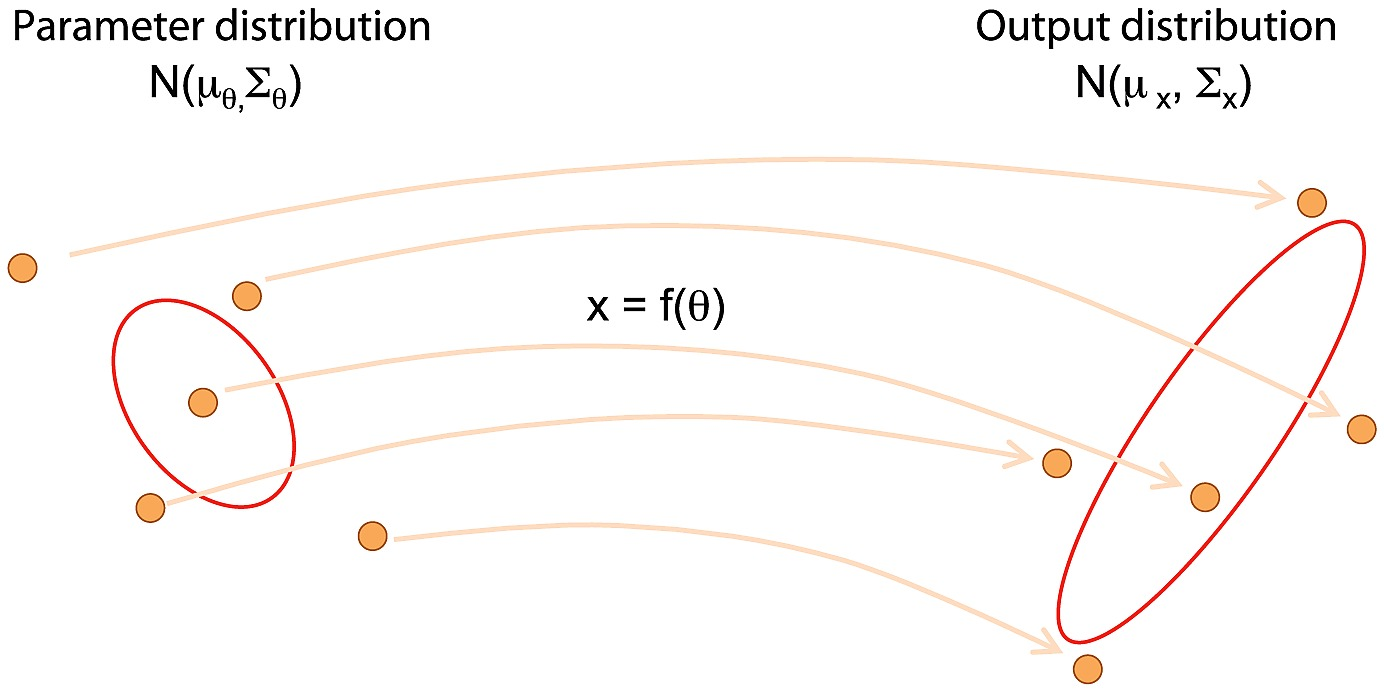
\includegraphics{unscented.jpg}
\caption{Unscented tranform}
\end{figure}

\paragraph{Kalman update}\label{kalman-update}

\[\mathbf{S} = \mathbf{H}_t \mathbf{\Sigma}^{-}_t \mathbf{H}_t^T + \mathbf{R}_t\]
\[\hat{\mathbf{z}} = h(\hat{\mathbf{x}}^{-}_t)\]
\[\mathbf{K} = \mathbf{\Sigma}^{-}_t \mathbf{H}_t^T \mathbf{S}^{-1}\]
\[\mathbf{\Sigma}_t = \mathbf{\Sigma}^-_t + \mathbf{K} \mathbf{S} \mathbf{K}^T\]
\[\hat{\mathbf{x}}_t = \hat{\mathbf{x}}^{-}_t + \mathbf{K}(\mathbf{z}_t - \hat{\mathbf{z}})\]

\subsection{F partial derivatives}\label{f-partial-derivatives}

\begin{Shaded}
\begin{Highlighting}[]
\NormalTok{Q.}\OperatorTok{<}\NormalTok{i,j,k}\OperatorTok{>} \OperatorTok{=}\NormalTok{ QuaternionAlgebra(SR, }\OperatorTok{-}\DecValTok{1}\NormalTok{, }\OperatorTok{-}\DecValTok{1}\NormalTok{)}

\NormalTok{var(}\StringTok{'q0, q1, q2, q3'}\NormalTok{)}
\NormalTok{var(}\StringTok{'dt'}\NormalTok{)}
\NormalTok{var(}\StringTok{'wx, wy, wz'}\NormalTok{)}

\NormalTok{q }\OperatorTok{=}\NormalTok{ q0 }\OperatorTok{+}\NormalTok{ q1}\OperatorTok{*}\NormalTok{i }\OperatorTok{+}\NormalTok{ q2}\OperatorTok{*}\NormalTok{j }\OperatorTok{+}\NormalTok{ q3}\OperatorTok{*}\NormalTok{k}

\NormalTok{w }\OperatorTok{=}\NormalTok{ vector([wx, wy, wz])}\OperatorTok{*}\NormalTok{dt}
\NormalTok{w_norm }\OperatorTok{=}\NormalTok{ sqrt(w[}\DecValTok{0}\NormalTok{]}\OperatorTok{^}\DecValTok{2} \OperatorTok{+}\NormalTok{ w[}\DecValTok{1}\NormalTok{]}\OperatorTok{^}\DecValTok{2} \OperatorTok{+}\NormalTok{ w[}\DecValTok{2}\NormalTok{]}\OperatorTok{^}\DecValTok{2}\NormalTok{)}
\NormalTok{ang }\OperatorTok{=}\NormalTok{ w_norm}\OperatorTok{/}\DecValTok{2}
\NormalTok{w_normalized }\OperatorTok{=}\NormalTok{ w}\OperatorTok{/}\NormalTok{w_norm}
\NormalTok{sin2 }\OperatorTok{=}\NormalTok{ sin(ang)}
\NormalTok{qd }\OperatorTok{=}\NormalTok{ cos(ang) }\OperatorTok{+}\NormalTok{ w_normalized[}\DecValTok{0}\NormalTok{]}\OperatorTok{*}\NormalTok{sin2}\OperatorTok{*}\NormalTok{i }\OperatorTok{+}\NormalTok{ w_normalized[}\DecValTok{1}\NormalTok{]}\OperatorTok{*}\NormalTok{sin2}\OperatorTok{*}\NormalTok{j }\OperatorTok{+}\NormalTok{ w_normalized[}\DecValTok{2}\NormalTok{]}\OperatorTok{*}\NormalTok{sin2}\OperatorTok{*}\NormalTok{k}

\NormalTok{nq }\OperatorTok{=}\NormalTok{ q}\OperatorTok{*}\NormalTok{qd}

\NormalTok{v }\OperatorTok{=}\NormalTok{ vector(nq.coefficient_tuple())}

\ControlFlowTok{for}\NormalTok{ sym }\KeywordTok{in}\NormalTok{ [wx, wy, wz, q0, q1, q2, q3]:}
\NormalTok{    d }\OperatorTok{=}\NormalTok{ diff(v, sym)}
\NormalTok{    exps }\OperatorTok{=} \BuiltInTok{map}\NormalTok{(}\KeywordTok{lambda}\NormalTok{ x: x.canonicalize_radical().full_simplify(), d)}
    \ControlFlowTok{for}\NormalTok{ i, e }\KeywordTok{in} \BuiltInTok{enumerate}\NormalTok{(exps):}
        \BuiltInTok{print}\NormalTok{(sym, i, e) }
        
\end{Highlighting}
\end{Shaded}

\subsection{Unscented Kalman Filters}\label{unscented-kalman-filters}

The EKF has 3 flaws in our case:

\begin{itemize}
\tightlist
\item
  The linearization gives an approximate form which result in
  approximation errors
\item
  The prediction step of the EKF assume that the linearized form of the
  transformation can capture all the information needed to apply the
  transformation to the gaussian distribution pre-transformation.
  Unfortunately, this is only true near the region of the mean. The
  transformation of the tail of the gaussian distribution may need to be
  very different.
\item
  It attempts to define a gaussian covariance matrix for the attitude
  quaternion. This does not make sense because it does not account for
  the requirement of the quaternion being in a 4 dimensional unit
  sphere.
\end{itemize}

The Unscented Kalman Filter (UKF) does not suffer from the two first
flaws, but it is more computationally expensive as it requires a
cholesky factorisation that grows exponentially in complexity with the
number of dimensions.

Indeed, the UKF applies an unscented transformation to sigma points of
the current approximated distribution. The statistics of the new
approximated gaussian are found through this unscented transform. The
EKF linearizes the transformation, the UKF approximates the resulting
gaussian after the transformation. Hence, the UKF can take into account
the effects of the transformation away from the mean which might be
drastically different.

The implementation of an UKF still suffer greatly from quaternion not
belonging to a vector space. The approach taken by
{[}\protect\hyperlink{ref-edgar_quaternion-based_nodate}{2}{]} is to use
the error quaternion defined by
\(\mathbf{e}_i = \mathbf{q}_i\bar{\mathbf{q}}\). This approach has the
benefit that similar quaternion differences result in similar error. But
apart from that, it does not have any profound justification. We must
compute a sound average weighted quaternion of all sigma points. An
algorithm is described in the following section.

\subsubsection{Average quaternion}\label{average-quaternion}

Unfortunately, the average of quaternions components
\(\frac{1}{N} \sum q_i\) or \emph{barycentric} mean is unsound: Indeed,
attitude do not belong to a vector space but a homogenous Riemannian
manifold (the four dimensional unit sphere). To convince yourself of the
unsoundness of the \emph{barycentric} mean, see that the addition and
barycentric mean of two unit quaternion is not necessarily an unit
quaternion (\((1, 0, 0, 0)\) and \((-1, 0, 0, 0)\) for instance.
Furthermore, angle being periodic, the \emph{barycentric} mean of a
quaternion with angle \(-178^\circ\) and another with same body-axis and
angle \(180^\circ\) gives \(1^\circ\) instead of the expected
\(-179^\circ\).

To calculate the average quaternion, we use an algorithm which minimize
a metric that correspond to the weighted attitude difference to the
average, namely the weighted sum of the squared Frobenius norms of
attitude matrix differences.
\[\bar{\mathbf{q}} = arg \min_{q \in \mathbb{S}^3} \sum w_i \| A(\mathbf{q}) - A(\mathbf{q}_i) \|^2_F\]

where \(\mathbb{S}^3\) denotes the unit sphere.

The attitude matrix \(A(\mathbf{q})\) and its corresponding Frobenius
norm have been described in the quaternion section.

\subsubsection{Intuition}\label{intuition}

The intuition of keeping track of multiple representative of the
distribution is exactly the approach taken by the particle filter. The
particle filter has the advantage that the distribution is never
transformed back to a gaussian so there is less assumption made about
the noise and the transformation. It is only required to be able to
calculate the expectation from a weighted set of particles.

\subsection{Particle Filter}\label{particle-filter}

Particle filters are sequential monte carlo methods. Like all monte
carlo method, they rely on repeated sampling for estimation of a
distribution.

\begin{figure}
\centering
\includegraphics{mc.gif}
\caption{Monte carlo estimation of pi}
\end{figure}

The particle filter itself a weighted particle representation of the
posterior:

\[p(\mathbf{x}) = \sum w^{(i)}\delta(\mathbf{x} - \mathbf{x}^{(i)})\]
where \(\delta\) is the dirac delta function. The dirac delta function
is zero everywhere except at zero, with an integral of one over the
entire real line. It represents here the ideal probability density of a
particle.

\subsubsection{Importance sampling}\label{importance-sampling}

The weights here come from importance sampling. It represents the fact
that each particle does not represent equally the distribution.
Importance sampling enables to use sampling from another distribution to
estimate properties from the target distribution of interest. In most
cases, it can be used to focus sampling on the region of interest. But
in our case, it enables us to reweight particles based on their
likelihood from the measurements.

Importance sampling is based on the identity:

\[
\begin{aligned}
\mathbb{E}[\mathbf{g}(\mathbf{x}) | \mathbf{y}_{1:T}] &= \int \mathbf{g}(\mathbf{x})p(\mathbf{x}|\mathbf{y}_{1:T})d\mathbf{x} \\
&= \int \left [\mathbf{g}(\mathbf{x})\frac{p(\mathbf{x}|\mathbf{y}_{1:T})}{\mathbf{\pi}(\mathbf{x}|\mathbf{y}_{1:T})} \right ] \mathbf{\pi}(\mathbf{x}|\mathbf{y}_{1:T}) d\mathbf{x} 
\end{aligned}
\]

\subsubsection{Sequential Importnce
Samplng}\label{sequential-importnce-samplng}

** TODO **

Particle filters are very computionally expensive and that is why their
usage is not very popular currently for low-powered embedded systems
like drones (But they are used in Avionics). Using accelerated hardware
is one way to enable them on drones.

\subsubsection{Resampling}\label{resampling}

When the number of effective particles is too low (\(N/10\)), we apply
systematic resampling. The idea behind resampling is simple. The
distribution is represented by a number of particles with different
weights. As time goes, the repartition of weights degenerate. A large
subset of particles ends up having negligible weight which make them
irrelevant. In the most extreme case, one particle represents the whole
distribution. To avoid that degeneration, when the weights are too
unbalanced, we resample from the weights distribution: pick N times
among the particle and assign them a weight of \(1/N\), each pick has
odd \(w_i\) to pick the particle \(p_i\). Thus, some particles with
large weights are splitted up into smaller clone particle and others
with small weight are never picked. This process is similar to
evolution, at each generation, the most promising branch survive and
replicate while the less promising die off.

A popular method for resampling is systematic sampling as described by
{[}\protect\hyperlink{ref-doucet_tutorial_2009}{3}{]}:

Sample \(U_1 \sim \mathcal{U} [0, \frac{1}{N} ]\) and define
\(U_i = U_1 + \frac{i-1 }{N}\) for \(i = 2, \ldots, N\)

\subsection{Rao-Blackwellized Particle
Filter}\label{rao-blackwellized-particle-filter}

\subsubsection{Introduction}\label{introduction-1}

Compared to a plain PF, RPBF leverage the linearity of some components
of the state by assuming our model gaussian conditionned on a latent
variable: Given the attitude \(q_t\), our model is linear. This is where
RPBF shines: We use particle filtering to estimate our latent variable,
the attitude, and we use the optimal kalman filter to estimate the state
variable.

This main inspiration from this approach is
{[}\protect\hyperlink{ref-vernaza_rao-blackwellized_2006}{4}{]}.
However, it differs by:

\begin{itemize}
\tightlist
\item
  adapt the filter to drones by taking into account that the system is
  too dynamic for assuming that the accelerometer simply output the
  gravity vector. This is solved by augmenting the state with the
  acceleration as shown later.
\item
  not use measurements of the IMU as control inputs (this is usually
  used for wheeled vehicles because of the drift from the wheels) but
  have both control inputs and measurements.
\item
  add an attitude sensor.
\end{itemize}

We introduce the latent variable \(\boldsymbol{\theta}\)

The latent variable \(\boldsymbol{\theta}\) has for sole component the
attitude: \[\boldsymbol{\theta} = (\mathbf{q})\]

\(q_t\) is estimated from the product of the attitude of all particles
\(\mathbf{\theta^{(i)}} = \mathbf{q}^{(i)}_t\) as the ``average''
quaternion \(\mathbf{q}_t = avgQuat(\mathbf{q}^n_t)\). \(x^n\)
designates the product of all n arbitrary particle.

The weight definition is:

\[w^{(i)}_t = \frac{p(\boldsymbol{\theta}^{(i)}_{0:t} | \mathbf{y}_{1:t})}{\pi(\boldsymbol{\theta}^{(i)}_{0:t} | \mathbf{y}_{1:t})}\]

From the definition, it is proovable that:

\[w^{(i)}_t \propto \frac{p(\mathbf{y}_t | \boldsymbol{\theta}^{(i)}_{0:t-1}, \mathbf{y}_{1:t-1})p(\boldsymbol{\theta}^{(i)}_t | \boldsymbol{\theta}^{(i)}_{t-1})}{\pi(\boldsymbol{\theta}^{(i)}_t | \boldsymbol{\theta}^{(i)}_{1:t-1}, \mathbf{y}_{1:t})} w^{(i)}_{t-1}\]

We choose the dynamic of the model as the importance distribution:

\[\pi(\boldsymbol{\theta}^{(i)}_t | \boldsymbol{\theta}^{(i)}_{1:t-1}, \mathbf{y}_{1:t}) = p(\boldsymbol{\theta}^{(i)}_t | \boldsymbol{\theta}^{(i)}_{t-1}) \]

Hence,

\[w^{(i)}_t \propto p(\mathbf{y}_t | \boldsymbol{\theta}^{(i)}_{0:t-1}, \mathbf{y}_{1:t-1}) w^{(i)}_{t-1}\]

We then sum all \(w^{(i)}_t\) to find the normalization constant and
retrieve the actual \(w^{(i)}_t\)

\subsubsection{State}\label{state-4}

\[\mathbf{x}_t = (\mathbf{v}_t, \mathbf{p}_t)^T\]

Initial state \(\mathbf{x}_0 = (\mathbf{0}, \mathbf{0}, \mathbf{0})\)

Initial covariance matrix
\(\mathbf{\Sigma}_{6 \times 6} = \epsilon \mathbf{I}_{6 \times 6}\)

\subsubsection{Latent variable}\label{latent-variable}

\[\mathbf{q}^{(i)}_{t+1} = \mathbf{q}^{(i)}_t*R2Q({\Delta t} (\mathbf{\boldsymbol{\omega}_G}_t+\mathbf{\boldsymbol{\omega}_G}^\epsilon_t))\]

\(\mathbf{\boldsymbol{\omega}_G}^\epsilon_t\) represents the error from
the control input and is sampled from
\(\mathbf{\boldsymbol{\omega}_G}^\epsilon_t \sim \mathcal{N}(\mathbf{0}, \mathbf{R}_{\mathbf{\boldsymbol{\omega}_G}_t })\)

Initial attitude \(\mathbf{q_0}\) is sampled such that the drone pitch
and roll are none (parralel to the ground) but the yaw is unknown and
uniformly distributed.

Note that \(\mathbf{q}(t+1)\) is known in the
\protect\hyperlink{model-dynamic}{model dynamic} because the model is
conditionned under \(\boldsymbol{\theta}^{(i)}_{t+1}\).

\subsubsection{Indoor Measurement model}\label{indoor-measurement-model}

\begin{enumerate}
\def\labelenumi{\arabic{enumi}.}
\tightlist
\item
  Position:
  \[\mathbf{p_V}(t) = \mathbf{p}(t)^{(i)} + \mathbf{p_V}^\epsilon_t\]
  where
  \(\mathbf{p_V}^\epsilon_t \sim \mathcal{N}(\mathbf{0}, \mathbf{R}_{\mathbf{p_V}_t })\)
\item
  Attitude:
  \[\mathbf{q_V}(t) = \mathbf{q}(t)^{(i)}*R2Q(\mathbf{q_V}^\epsilon_t)\]
  where
  \(\mathbf{q_V}^\epsilon_t \sim \mathcal{N}(\mathbf{0}, \mathbf{R}_{\mathbf{q_V}_t })\)
\end{enumerate}

\subsubsection{Kalman prediction}\label{kalman-prediction-1}

The model dynamics define the following model, state-transition matrix
\(\mathbf{F}_t\{\boldsymbol{\theta}^{(i)}_t\}\), the control-input
matrix \(\mathbf{B}_t\{\boldsymbol{\theta}^{(i)}_t\}\), the process
noise \(\mathbf{w}_t\{\boldsymbol{\theta}^{(i)}_t\}\) for the Kalman
filter and its covariance
\(\mathbf{Q}_t\{\boldsymbol{\theta}^{(i)}_t\}\)

\[\mathbf{x}_t = \mathbf{F}_t\{\boldsymbol{\theta}^{(i)}_t\} \mathbf{x}_{t-1} + \mathbf{B}_t\{\boldsymbol{\theta}^{(i)}_t\} \mathbf{u}_t + \mathbf{w}_t\{\boldsymbol{\theta}^{(i)}_t\}\]

\[\mathbf{F}_t\{\boldsymbol{\theta}^{(i)}_t\}_{6 \times 6} = 
\left( \begin{array}{cc}
\mathbf{I}_{3 \times 3} & 0 \\
\Delta t~\mathbf{I}_{3 \times 3} & \mathbf{I}_{3 \times 3}
\end{array} \right)\]

\[\mathbf{B}_t\{\boldsymbol{\theta}^{(i)}_t\}_{6 \times 3} = 
\left( \begin{array}{c}
\mathbf{R}_{b2f}\{\mathbf{q}^{(i)}_{t}\}\mathbf{a_A} \\
\mathbf{0}_{3 \times 3} \\
\end{array} \right)\]

\[\mathbf{Q}_t\{\boldsymbol{\theta}^{(i)}_t\}_{6 \times 6} = 
\left( \begin{array}{cc}
\mathbf{R}_{b2f}\{\mathbf{q}^{(i)}_{t}\}(\mathbf{Q}_{\mathbf{a}_t } * dt^2)\mathbf{R}^t_{b2f}\{\mathbf{q}^{(i)}_{t}\} & \\
& \mathbf{Q}_{\mathbf{v}_t }\\
\end{array} \right)\]

\[\hat{\mathbf{x}}^{-(i)}_t = \mathbf{F}_t\{\boldsymbol{\theta}^{(i)}_t\} \mathbf{x}^{(i)}_{t-1} + \mathbf{B}_t\{\boldsymbol{\theta}^{(i)}_t\} \mathbf{u}_t \]
\[ \mathbf{\Sigma}^{-(i)}_t = \mathbf{F}_t\{\boldsymbol{\theta}^{(i)}_t\} \mathbf{\Sigma}^{-(i)}_{t-1}  (\mathbf{F}_t\{\boldsymbol{\theta}^{(i)}_t\})^T + \mathbf{Q}_t\{\boldsymbol{\theta}^{(i)}_t\}\]

\subsubsection{Kalman measurement
update}\label{kalman-measurement-update}

The \protect\hyperlink{measurements-model-1}{measurement model} defines
how to compute
\(p(\mathbf{y}_t | \boldsymbol{\theta}^{(i)}_{0:t-1}, \mathbf{y}_{1:t-_K1})\)

Indeed, The measurement model defines the observation matrix
\(\mathbf{H}_t\{\boldsymbol{\theta}^{(i)}_t\}\), the observation noise
\(\mathbf{v}_t\{\boldsymbol{\theta}^{(i)}_t\}\) and its covariance
matrix \(\mathbf{R}_t\{\boldsymbol{\theta}^{(i)}_t\}\) for the Kalman
filter.

\[(\mathbf{a_A}_t, \mathbf{p_V}_t)^T  = \mathbf{H}_t\{\boldsymbol{\theta}^{(i)}_t\} (\mathbf{v}_t, \mathbf{p}_t)^T + \mathbf{v}_t\{\boldsymbol{\theta}^{(i)}_t\}\]

\[\mathbf{H}_t\{\boldsymbol{\theta}^{(i)}_t\}_{6 \times 3} = 
\left( \begin{array}{cc}
\mathbf{0}_{3 \times 3} & \\
& \mathbf{I}_{3 \times 3} \\
\end{array} \right)\]

\[\mathbf{R}_t\{\boldsymbol{\theta}^{(i)}_t\}_{3 \times 3} = 
\left( \begin{array}{c}
\mathbf{R}_{\mathbf{p_V}_t} 
\end{array} \right)\]

\subsubsection{Kalman update}\label{kalman-update-1}

\[\mathbf{S} = \mathbf{H}_t\{\boldsymbol{\theta}^{(i)}_t\} \mathbf{\Sigma}^{-(i)}_t  (\mathbf{H}_t\{\boldsymbol{\theta}^{(i)}_t\})^T + \mathbf{R}_t\{\boldsymbol{\theta}^{(i)}_t\}\]
\[\hat{\mathbf{z}} = \mathbf{H}_t\{\boldsymbol{\theta}^{(i)}_t\}  \hat{\mathbf{x}}^{-(i)}_t\]
\[\mathbf{K} = \mathbf{\Sigma}^{-(i)}_t \mathbf{H}_t\{\boldsymbol{\theta}^{(i)}_t\}^T \mathbf{S}^{-1}\]
\[\mathbf{\Sigma}^{(i)}_t = \mathbf{\Sigma}^{-(i)}_t + \mathbf{K} \mathbf{S} \mathbf{K}^T\]
\[\hat{\mathbf{x}}^{(i)}_t = \hat{\mathbf{x}}^{-(i)}_t  + \mathbf{K}((\mathbf{a_A}_t, \mathbf{p_V}_t)^T - \hat{\mathbf{z}})\]
\[p(\mathbf{y}_t | \boldsymbol{\theta}^{(i)}_{0:t-1}, \mathbf{y}_{1:t-1}) = \mathcal{N}((\mathbf{a_A}_t, \mathbf{p_V}_t)^T; \hat{\mathbf{z}}_t, \mathbf{S})\]

\subsubsection{Asynchronous
measurements}\label{asynchronous-measurements}

Our measurements might have different sampling rate so instead of doing
full kalman update, we only apply a partial kalman update corresponding
to the current type of measurement \(\mathbf{z}_t\).

For indoor, there is only one kind of sensor for the Kalman update:
\(\mathbf{p_V}\)

\subsubsection{Attitude reweighting}\label{attitude-reweighting}

In the \protect\hyperlink{measurements-model}{measurement model}, the
attitude defines another reweighting for importance sampling.

\[p(\mathbf{y}_t | \boldsymbol{\theta}^{(i)}_{0:t-1}, \mathbf{y}_{1:t-1}) = \mathcal{N}(Q2R({\mathbf{q}^{(i)}}^{-1}\mathbf{q_V}_t);~ 0 ,~ \mathbf{R}_{\mathbf{q_V}})\]

\subsection{Algorithm summary}\label{algorithm-summary}

\begin{enumerate}
\def\labelenumi{\arabic{enumi}.}
\tightlist
\item
  Initiate \(N\) particles with \(\mathbf{x}_0\),
  \(\mathbf{q}_0 ~ \sim p(\mathbf{q}_0)\), \(\mathbf{\Sigma}_0\) and
  \(w = 1/N\)
\item
  While new sensor measurements \((\mathbf{z}_t, \mathbf{u}_t)\)
\end{enumerate}

\begin{itemize}
\tightlist
\item
  foreach \(N\) particles \((i)\):

  \begin{enumerate}
  \def\labelenumi{\arabic{enumi}.}
  \tightlist
  \item
    Depending on the type of observation:

    \begin{itemize}
    \tightlist
    \item
      \textbf{IMU}:

      \begin{enumerate}
      \def\labelenumii{\arabic{enumii}.}
      \tightlist
      \item
        store \(\boldsymbol{\mathbf{\omega_G}}_t\) and
        \(\mathbf{a_A}_t\) as last control inputs
      \item
        sample new latent variable \(\boldsymbol{\theta_t}\) from
        \(\boldsymbol{\mathbf{\omega_G}}_t\) (which correspond to the
        last control inputs)
      \item
        apply kalman prediction from \(\mathbf{a_A}_t\) (which
        correspond to the last control inputs)
      \end{enumerate}
    \item
      \textbf{Vicon}:

      \begin{enumerate}
      \def\labelenumii{\arabic{enumii}.}
      \tightlist
      \item
        sample new latent variable \(\boldsymbol{\theta_t}\) from
        \(\boldsymbol{\mathbf{\omega_G}}_t\) (which correspond to the
        last control inputs)
      \item
        apply kalman prediction from \(\mathbf{a_A}_t\) (which
        correspond to the last control inputs)
      \item
        Partial kalman update with:
        \[\mathbf{H}_t\{\boldsymbol{\theta}^{(i)}_t\}_{3 \times 6} = (\mathbf{0}_{3 \times 3} ~~~~ \mathbf{I}_{3 \times 3} )\]
        \[\mathbf{R}_t\{\boldsymbol{\theta}^{(i)}_t\}_{3 \times 3} =  \mathbf{R}_{\mathbf{p_V}_t }\]
        \[\mathbf{x}^{(i)}_t = \mathbf{H}_t\{\boldsymbol{\theta}^{(i)}_t\} \mathbf{x}^{(i)}_{t-1} + \mathbf{K}(\mathbf{p_V}_t - \hat{\mathbf{z}})\]
        \[p(\mathbf{y}_t | \boldsymbol{\theta}^{(i)}_{0:t-1}, \mathbf{y}_{1:t-1}) = \mathcal{N}(\mathbf{q_V}_t; \mathbf{q}^{(i)}_t,~ \mathbf{R}_{\mathbf{q_V}_t } )\mathcal{N}(\mathbf{p_V}_t; \hat{\mathbf{z}}_t, \mathbf{S})\]
      \end{enumerate}
    \item
      \textbf{Other sensors (Outdoor)}: As for \textbf{Vicon} but use
      the corresponding partial kalman update
    \end{itemize}
  \item
    Update \(w^{(i)}_t\):
    \(w^{(i)}_t = p(\mathbf{y}_t | \boldsymbol{\theta}^{(i)}_{0:t-1}, \mathbf{y}_{1:t-1}) w^{(i)}_{t-1}\)\\
  \end{enumerate}
\item
  Normalize all \(w^{(i)}\) by scalaing by \(1/(\sum w^{(i)})\) such
  that \(\sum w^{(i)}= 1\)
\item
  Compute \(\mathbf{p}_t\) and \(\mathbf{q}_t\) as the expectation from
  the distribution approximated by the N particles.
\item
  Resample if the number of effective particle is too low
\end{itemize}

\subsubsection{Extension to outdoors}\label{extension-to-outdoors}

As highlighted in the Algorithm summary, the RPBF if easily extensible
to other sensors. Indeed, measurements are either:

\begin{itemize}
\tightlist
\item
  giving information about position or velocity and their update is
  similar to the vicon position update as a kalman partial update
\item
  giving information about the orientation and their update is similar
  to the vicon attitude update as a pure importance sampling
  reweighting.
\end{itemize}

As a proof-of-conceptalternative Rao-blackwellized particle filter
specialized for outdoor has been developped that integrates the
following sensors:

\begin{itemize}
\tightlist
\item
  IMU with accelerometer, gyroscope \textbf{and magnetometer}
\item
  Altimeter
\item
  Dual GPS (2 GPS)
\item
  Optical Flow
\end{itemize}

The optical flow measurements are assumed to be of the form
\((\Delta \mathbf{p}, \Delta \mathbf{q})\) for a \(\Delta t\)
corresponding to its sampling rate. It is inputed to the particle filter
as a likelihood:

\[p(\mathbf{y}_t | \boldsymbol{\theta}^{(i)}_{0:t-1}, \mathbf{y}_{1:t-1}) = \mathcal{N}(\mathbf{p}_{t1} + \Delta p; \mathbf{p}_{t2}; \mathbf{R}_{\mathbf{dp_O}_t})\mathcal{N}(\Delta \mathbf{q}; \mathbf{q}_{t1}^{-1}\mathbf{q}_{t2}; \mathbf{R}_{\mathbf{dq_O}_t})\]

where \(t2 = t1 + \Delta t\), \(\mathbf{p}_{t2}\) is the latest kalman
prediction and \(\mathbf{q}_{t2}\) is the latest latent variable through
sampling of the attitude updates.

\subsection{Results}\label{results}

\textbf{TODO}

Parameters used

Table of RMSE

Graph that shows the tracking through time

\subsection{Conclusion}\label{conclusion}

\textbf{TODO}

\section{Pt II: A simulation tool for scala with spatial integration:
scala-flow}\label{pt-ii-a-simulation-tool-for-scala-with-spatial-integration-scala-flow}

\subsection{Purpose}\label{purpose}

\subsection{Source, Sink and
Transformations}\label{source-sink-and-transformations}

\subsection{Flow graphical
representation}\label{flow-graphical-representation}

\subsection{Buffer and cycles}\label{buffer-and-cycles}

\subsection{Data}\label{data}

\subsection{Source API}\label{source-api}

\subsubsection{FP}\label{fp}

Here is a simplified description of the API of each source.

\begin{Shaded}
\begin{Highlighting}[]

\KeywordTok{trait}\NormalTok{ Source[A] \{}

    \KeywordTok{def} \FunctionTok{foreach}\NormalTok{(f: A => Unit): Source[A]}
    \KeywordTok{def} \FunctionTok{foreachT}\NormalTok{(f: Timestamped[A] => Unit): Source[A]}
    
    \KeywordTok{def} \FunctionTok{filter}\NormalTok{(b: A => Boolean): Source[A]}
    \KeywordTok{def} \FunctionTok{filterT}\NormalTok{(b: Timestamped[Boolean]): Source[A] }
    
    \KeywordTok{def} \FunctionTok{takeWhile}\NormalTok{(b: A => Boolean): Source[A]}
    \KeywordTok{def} \FunctionTok{takeWhileT}\NormalTok{(b: Timestamped[A] => Boolean): Source[A] }
    
    \KeywordTok{def} \FunctionTok{drop}\NormalTok{(n: Int): Source[A]     }
    
    \KeywordTok{def}\NormalTok{ muted: Source[A]    }
    
    \KeywordTok{def} \FunctionTok{accumulate}\NormalTok{(clock: Source[Time]): Source[ListT[A]]}
    
    \KeywordTok{def}\NormalTok{ reduce[B](default: B, f: (B, B) => B)}
\NormalTok{        (}\KeywordTok{implicit}\NormalTok{ ev: A <:< ListT[B]): Source[B]}
    \KeywordTok{def}\NormalTok{ reduceT[B](default: B,}
\NormalTok{                  f: (Timestamped[B], Timestamped[B]) => Timestamped[B])}
\NormalTok{        (}\KeywordTok{implicit}\NormalTok{ ev: A <:< List[Timestamped[B]]): Source[B]}

    \KeywordTok{def}\NormalTok{ groupBy[B](f: A => B): Source[(B, A)]}
    \KeywordTok{def}\NormalTok{ groupByT[B](f: Timestamped[A] => B): Source[(B, A)] }
  
    \KeywordTok{def} \FunctionTok{debug}\NormalTok{(): Source[A]}

    \CommentTok{//USE ONLY WHEN THERE IS NO LOOP INVOLVED}
    \KeywordTok{def} \FunctionTok{buffer}\NormalTok{(init: A): Buffer[A]}

    \CommentTok{//Get old A but with the time of the new A}
    \KeywordTok{def} \FunctionTok{bufferWithTime}\NormalTok{(init: A): Buffer[A]}

    \KeywordTok{def}\NormalTok{ map[B](f: A => B): Source[B]}
    \KeywordTok{def}\NormalTok{ mapT[B](f: Timestamped[A] => B): Source[B]}

    \KeywordTok{def}\NormalTok{ flatMap[C](f: A => List[C]): Source[C]}
    \KeywordTok{def}\NormalTok{ flatMapT[C](f: Timestamped[A] => List[Timestamped[C]]): Source[C]   }

    \CommentTok{//Divide the frequency of the stream by n}
    \KeywordTok{def} \FunctionTok{divider}\NormalTok{(n: Int)}

    \CommentTok{//Zip everthing}
    \CommentTok{// A1 A2 B1 A3 B2 B3 B4 B5 A4}
    \CommentTok{// => (A1, B1), (A2, B2), (A3, B3), (A4, B4), [Queue[B5]]}
    \KeywordTok{def}\NormalTok{ zip[B](s2: Source[B])   }
    \KeywordTok{def}\NormalTok{ zipT[B](s2: Source[B])}

    \KeywordTok{def}\NormalTok{ unzip2[B, C](}\KeywordTok{implicit}\NormalTok{ ev: A <:< (B, C)): (Source[B], Source[C]) }

    \CommentTok{//Only zip the last of the right}
    \CommentTok{// A1 A2 B1 A3 B2 B3 B4 B5 A4=> (A1, B1), (A2, B2), (A3, B3), (A4, B5)}
    \KeywordTok{def}\NormalTok{ zipLastRight[B](s2: Source[B])}
\NormalTok{        : Source[(Timestamped[A], Timestamped[B])]  }
    \KeywordTok{def}\NormalTok{ zipLastRightT[B](s2: Source[B])}
\NormalTok{        : Source[(Timestamped[A], Timestamped[B])]  }
    
    \CommentTok{//Only zip the last pair}
    \CommentTok{// A1 A2 B1 A3 B2 B3 A4=> (A1, B1), (A3, B2), (B3, A4)}
    \KeywordTok{def}\NormalTok{ zipLast[B](s2: Source[B])}
\NormalTok{        : Source[(Timestamped[A], Timestamped[B])]  }
    \KeywordTok{def}\NormalTok{ zipLastT[B](s2: Source[B])}
\NormalTok{        : Source[(Timestamped[A], Timestamped[B])]  }
  
    \KeywordTok{def}\NormalTok{ merge[B](s2: Source[B]): Source[Either[A, B]]}
    
    \KeywordTok{def} \FunctionTok{fusion}\NormalTok{(sources: Source[A]*): Source[A]}
    
    \KeywordTok{def} \FunctionTok{latency}\NormalTok{(dt: Time): Source[A]}
    
    \KeywordTok{def}\NormalTok{ toTime: Source[Time]}

\NormalTok{\}}

\KeywordTok{class} \FunctionTok{TimeSource}\NormalTok{(source: Source[Time]) \{}

  \KeywordTok{def} \FunctionTok{stop}\NormalTok{(tf: Timeframe): Source[Time]}

  \KeywordTok{def} \FunctionTok{latencyVariance}\NormalTok{(mean: Real, std: Real): Source[Time]}
  
  \KeywordTok{def} \FunctionTok{latency}\NormalTok{(dt: Time): Source[Time] }
  
  \KeywordTok{def} \FunctionTok{deltaTime}\NormalTok{(init: Time = }\FloatTok{0.0}\NormalTok{): Source[Time]}
  
\NormalTok{\}}

\KeywordTok{class}\NormalTok{ DataSource[A: Data](source: Source[A]) \{}

  \KeywordTok{def} \FunctionTok{labelData}\NormalTok{(f: Time => A): Source[LabeledData[A]]}
  
\NormalTok{\}}
\end{Highlighting}
\end{Shaded}

The real API includes also a name and silent parameter. Both are useful
for the graphical representation. The name of the block will be
overriden by name if present and it will be skipped if silent is
present.

\subsection{Block}\label{block}

\subsection{Scheduling}\label{scheduling}

\subsection{Batch}\label{batch}

\subsection{Replay}\label{replay}

\subsection{Spatial integration}\label{spatial-integration}

\subsection{Conclusion}\label{conclusion-1}

\textbf{TODO}

\subsection{References}\label{references}

\section{An interpreter for spatial}\label{an-interpreter-for-spatial}

\subsection{Spatial}\label{spatial-1}

\section{Spatial implementation of a Rao-Blackwellized Particle
Filter}\label{spatial-implementation-of-a-rao-blackwellized-particle-filter}

\subsection{Spatial}\label{spatial-2}

\section*{Conclusion}\label{conclusion-2}
\addcontentsline{toc}{section}{Conclusion}

\section*{References}\label{references-1}
\addcontentsline{toc}{section}{References}

\hypertarget{refs}{}
\hypertarget{ref-markley_averaging_2007}{}
{[}1{]} F. L. Markley, Y. Cheng, J. L. Crassidis, and Y. Oshman,
``Averaging quaternions,'' \emph{Journal of Guidance, Control, and
Dynamics}, vol. 30, no. 4, pp. 1193--1197, 2007.

\hypertarget{ref-edgar_quaternion-based_nodate}{}
{[}2{]} K. Edgar, ``A Quaternion-based Unscented Kalman Filter for
Orientation Tracking.''.

\hypertarget{ref-doucet_tutorial_2009}{}
{[}3{]} A. Doucet and A. M. Johansen, ``A tutorial on particle filtering
and smoothing: Fifteen years later,'' \emph{Handbook of nonlinear
filtering}, vol. 12, nos. 656-704, p. 3, 2009.

\hypertarget{ref-vernaza_rao-blackwellized_2006}{}
{[}4{]} P. Vernaza and D. D. Lee, ``Rao-Blackwellized particle filtering
for 6-DOF estimation of attitude and position via GPS and inertial
sensors,'' in \emph{Robotics and Automation, 2006. ICRA 2006.
Proceedings 2006 IEEE International Conference on}, 2006, pp.
1571--1578.

\end{document}
